\section{Assumptions}
\begin{figure}[htb]
\centering
%\subfloat[side view]{
%	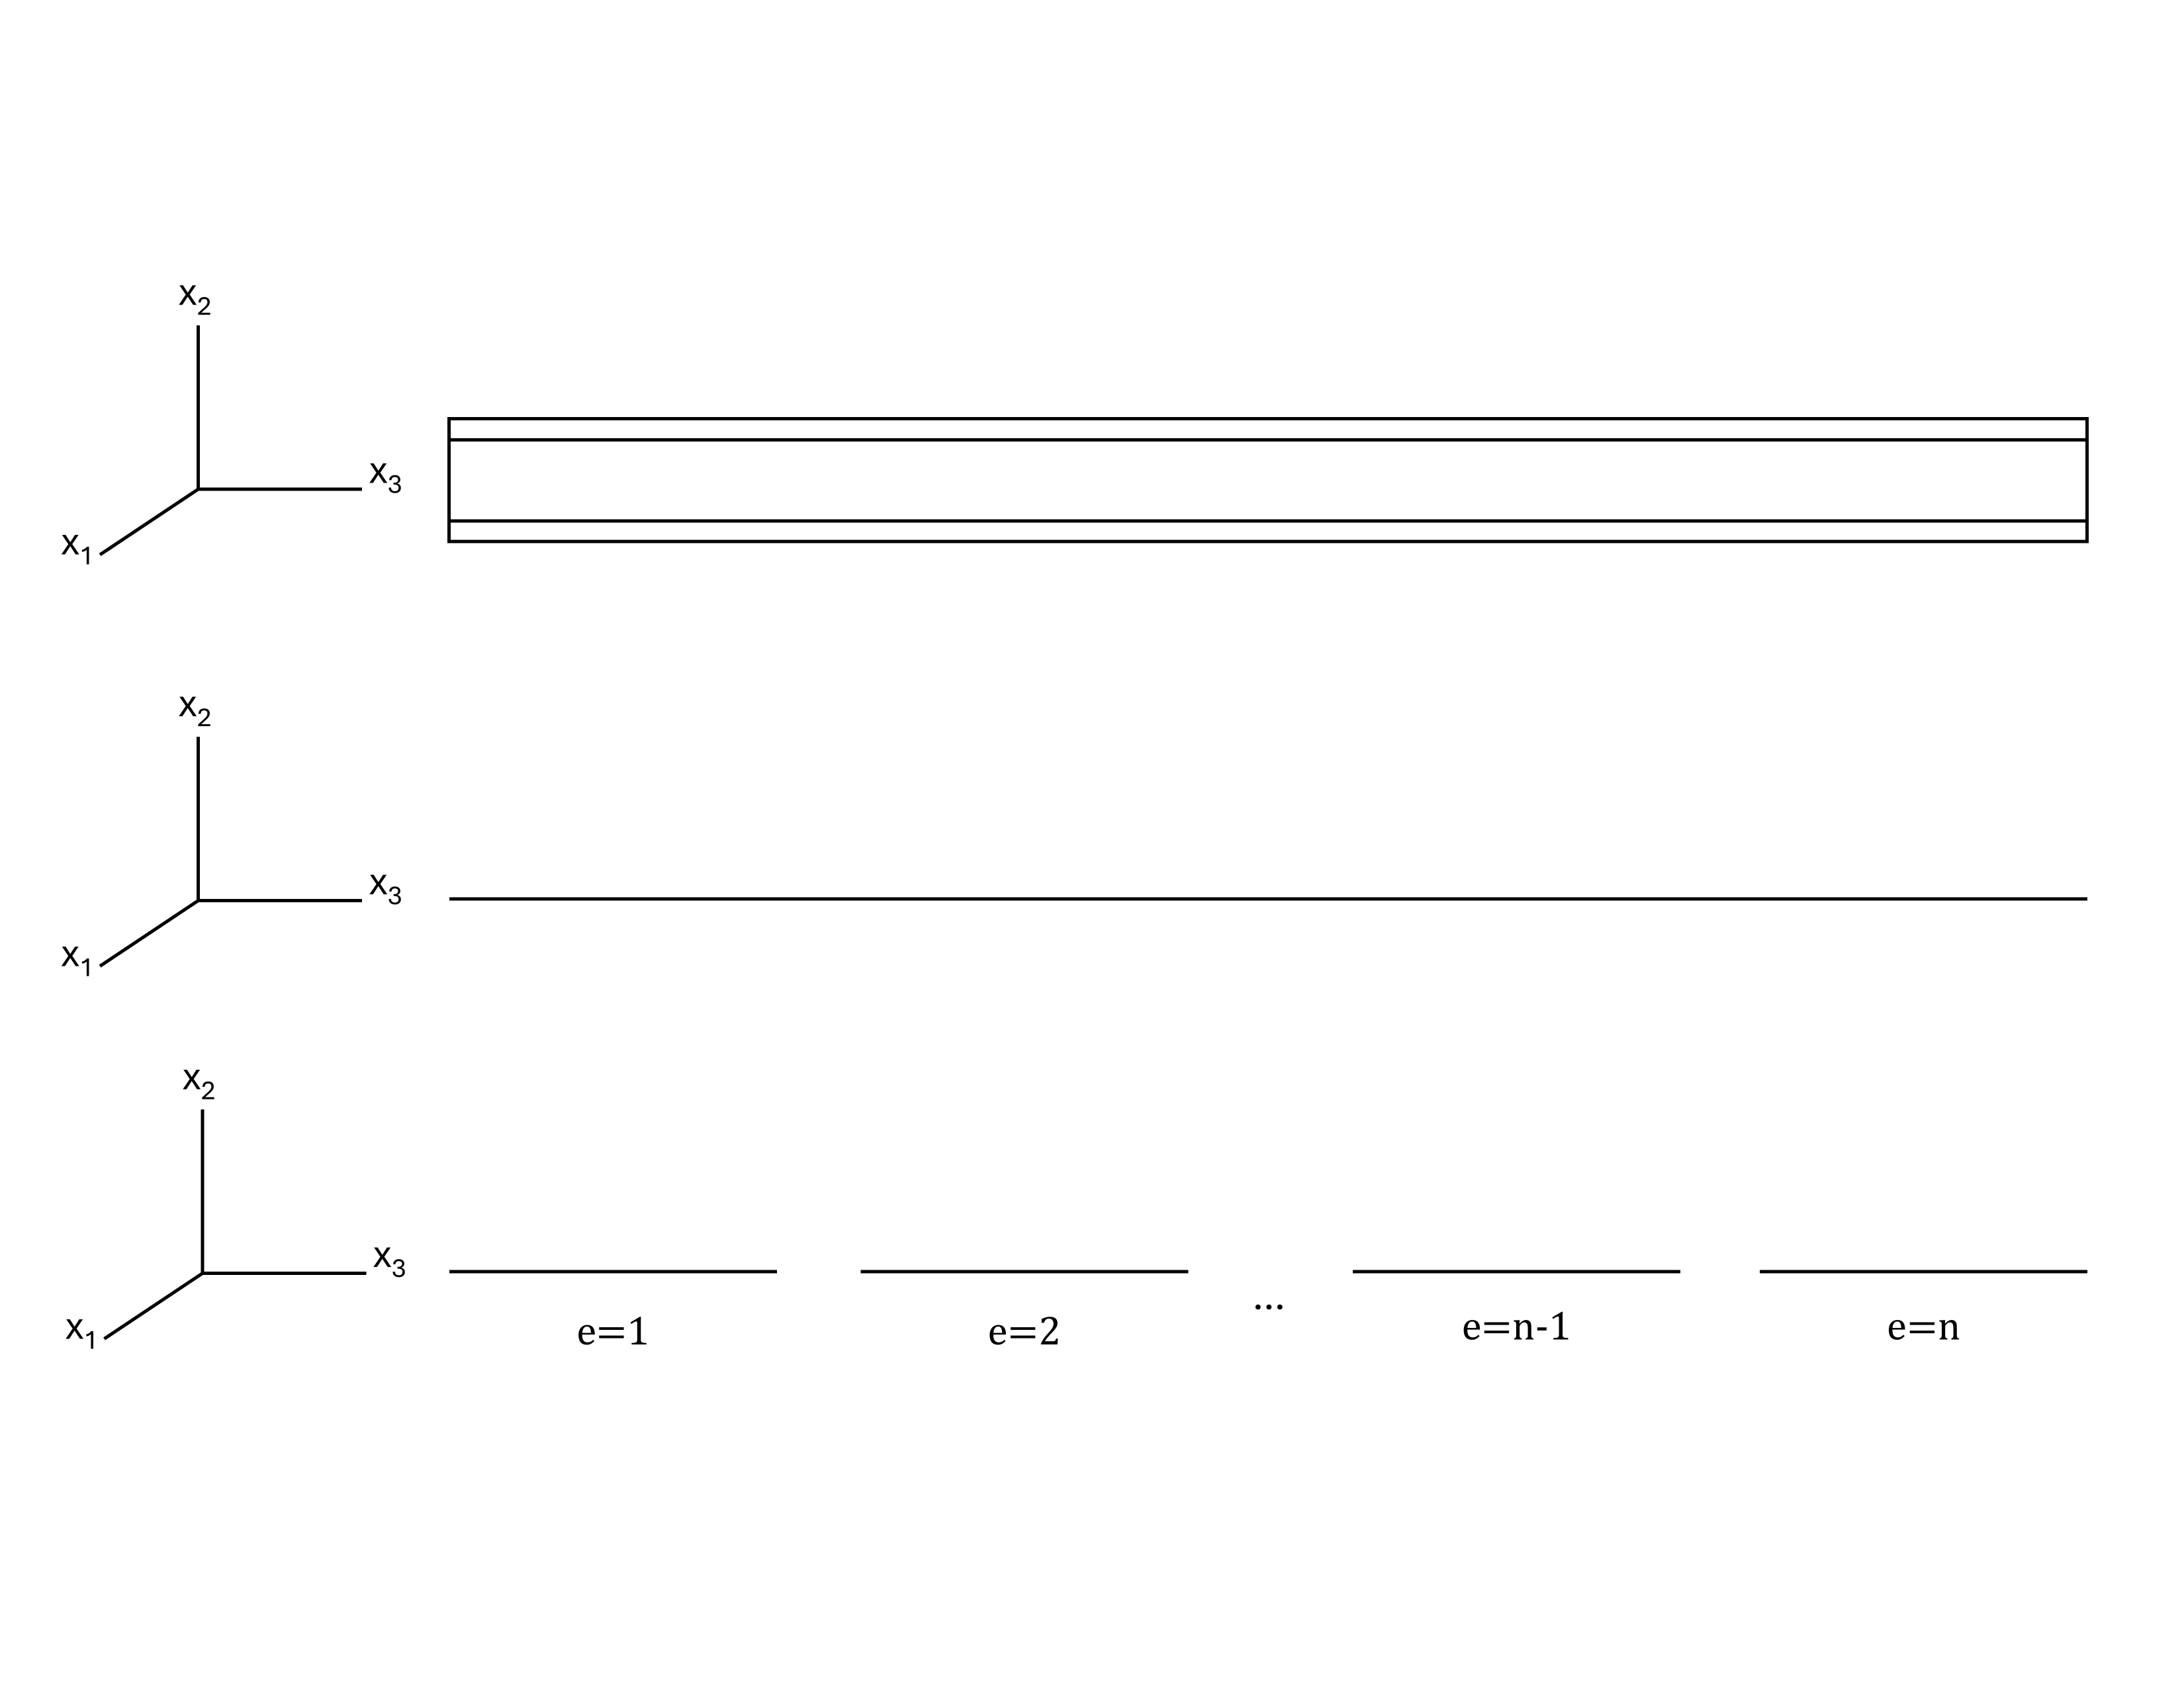
\includegraphics[width=0.7\columnwidth,trim=5.25cm 13cm 0cm 0cm, clip]{figs/beam_to_elements.png}
%}
%\centering
%\subfloat[isometric view]{
%	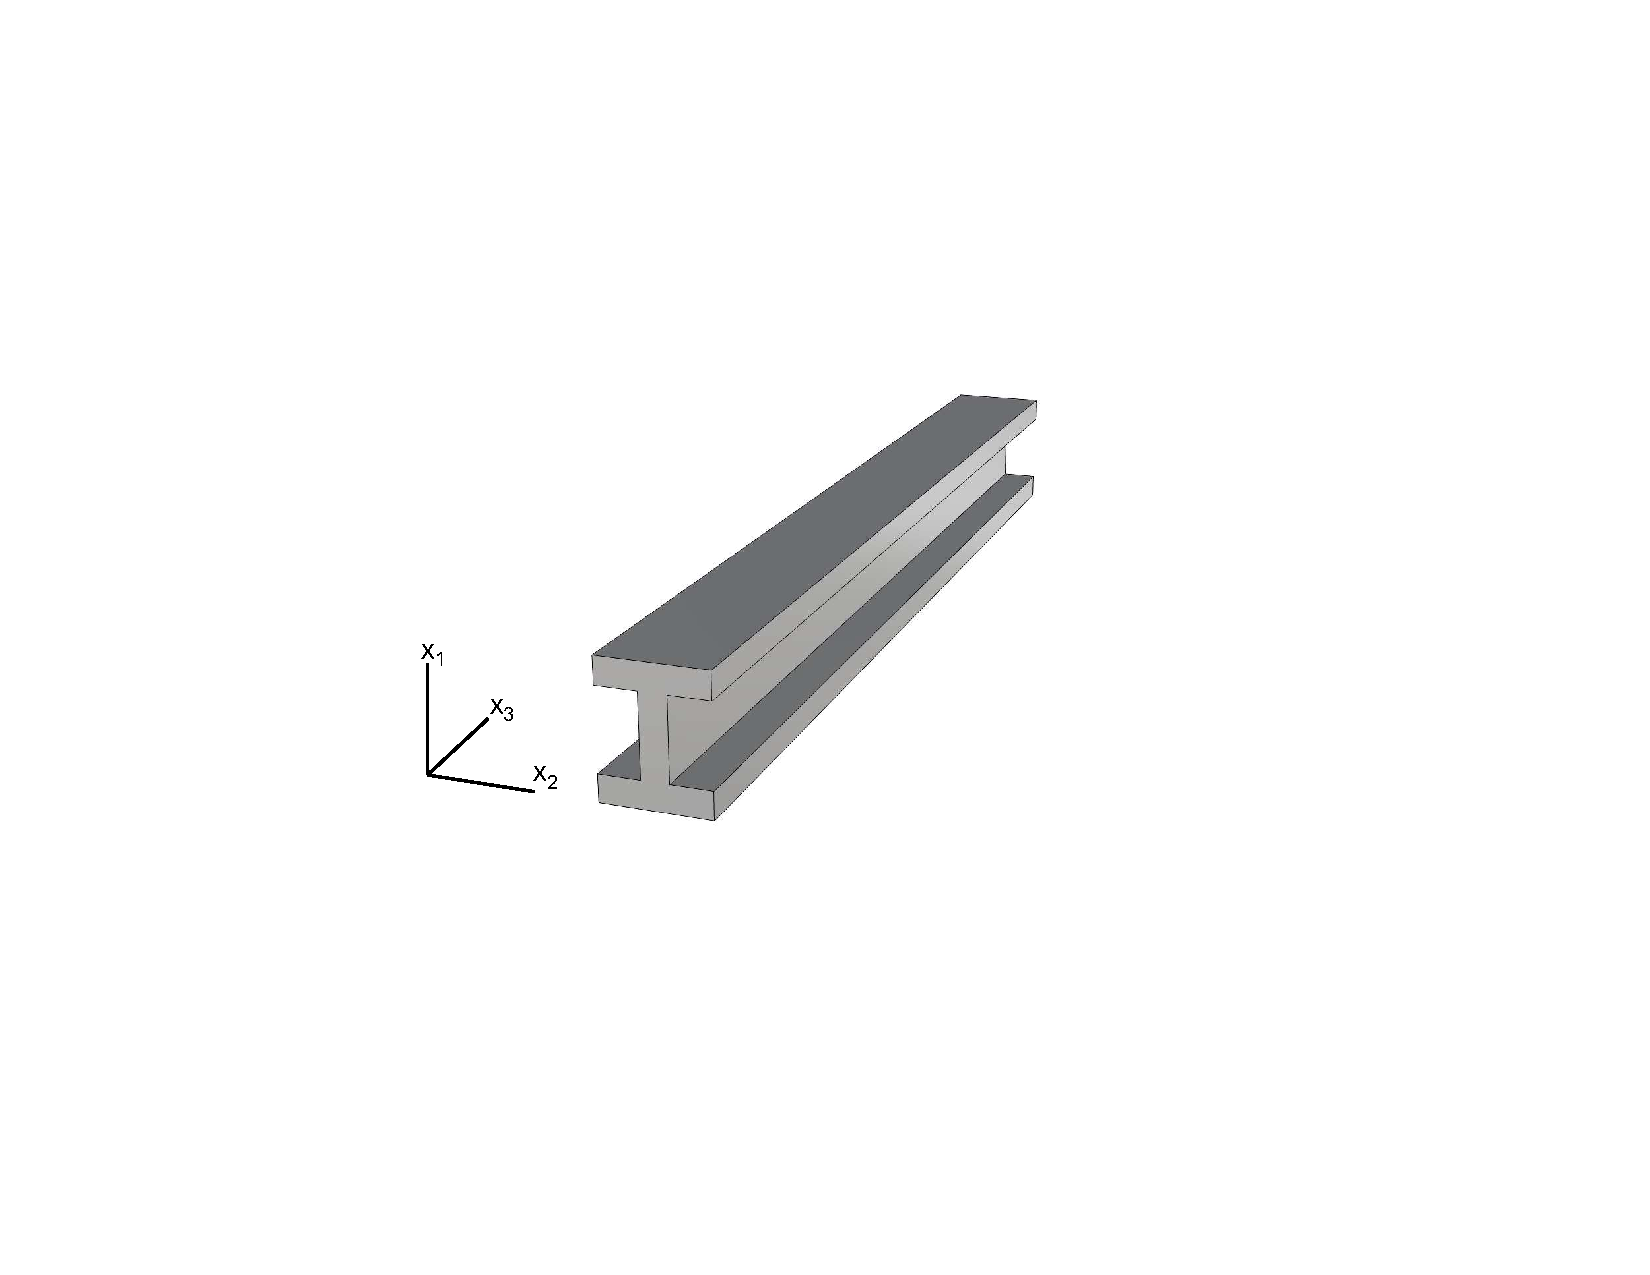
\includegraphics[width=0.25\columnwidth,trim=0cm 3cm 0cm 0cm, clip]{figs/straight.pdf}
%}
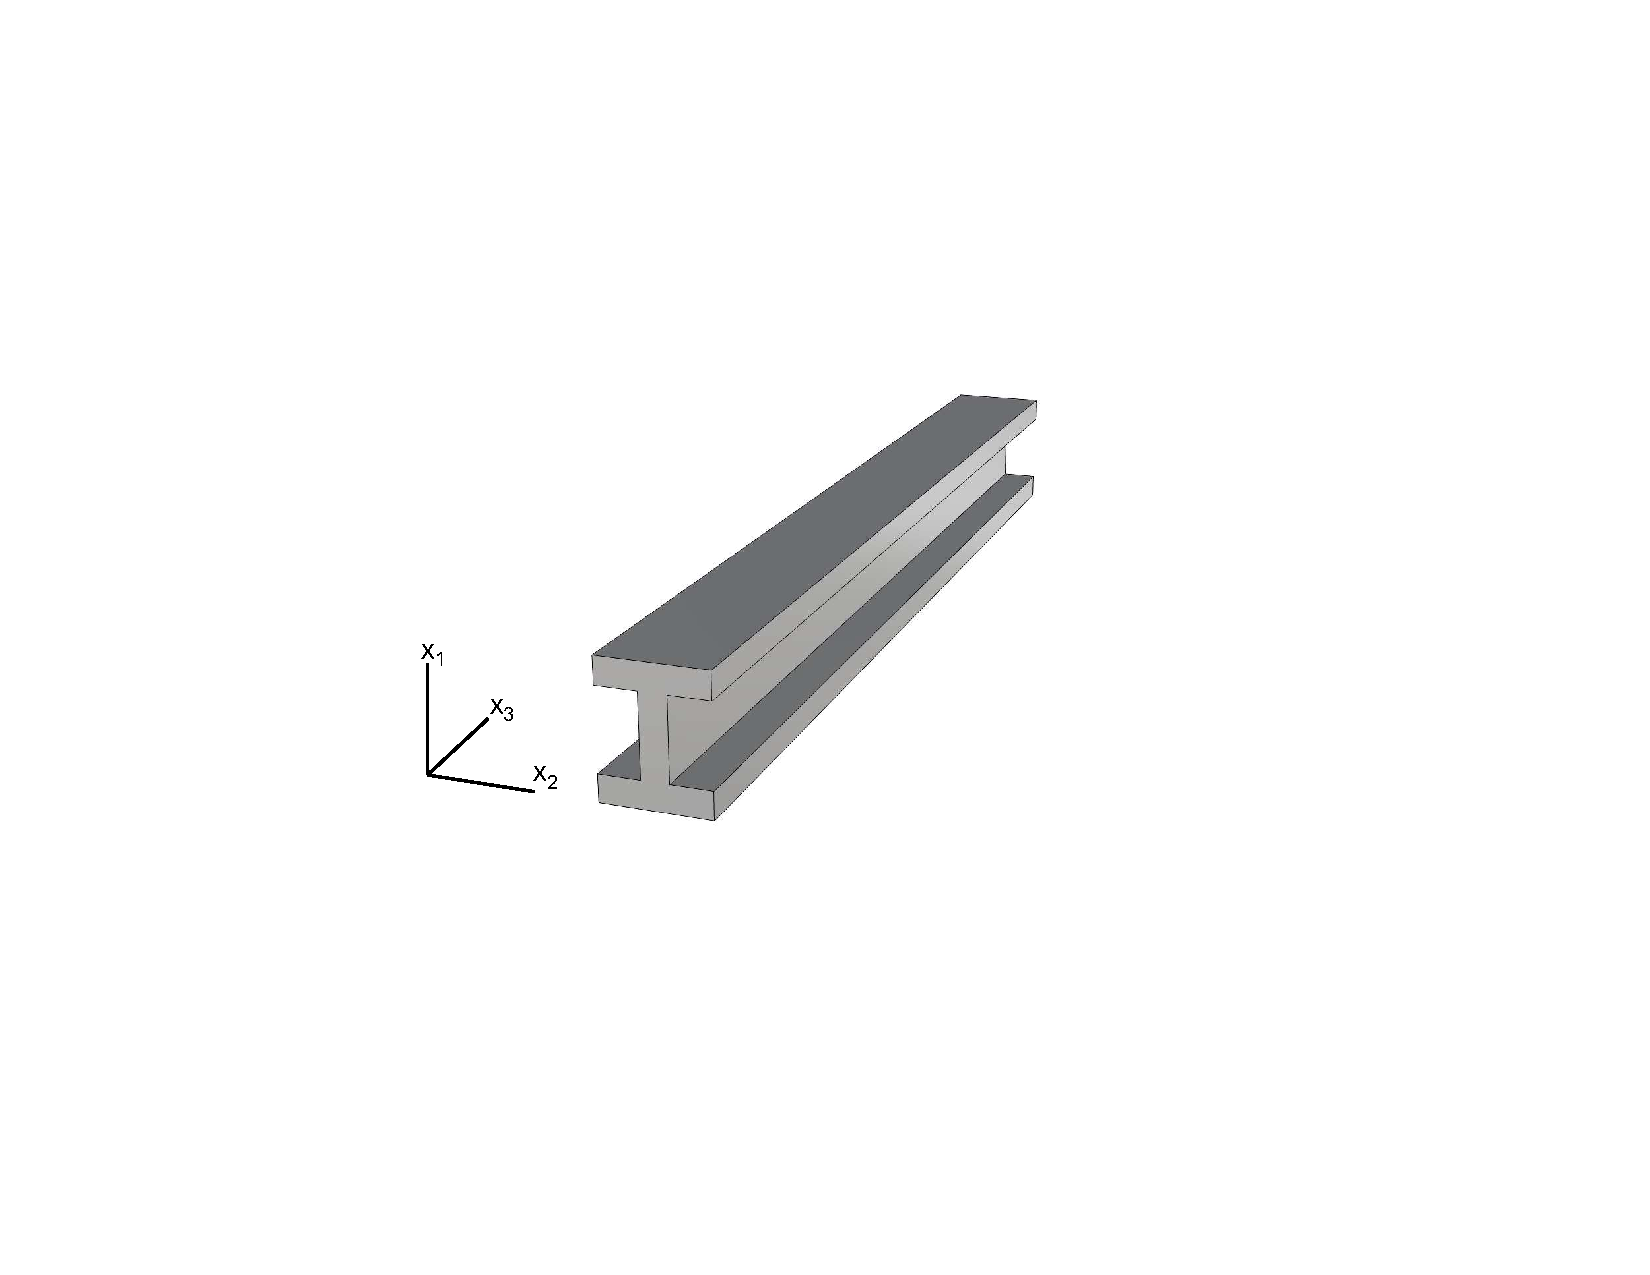
\includegraphics[width=0.95\columnwidth,trim=4cm 7cm 6cm 6.5cm, clip]{figs/straight.pdf}
\caption{The definition of the beam}
 \label{fig:beam_definition}
\end{figure}


\begin{figure}
\centering
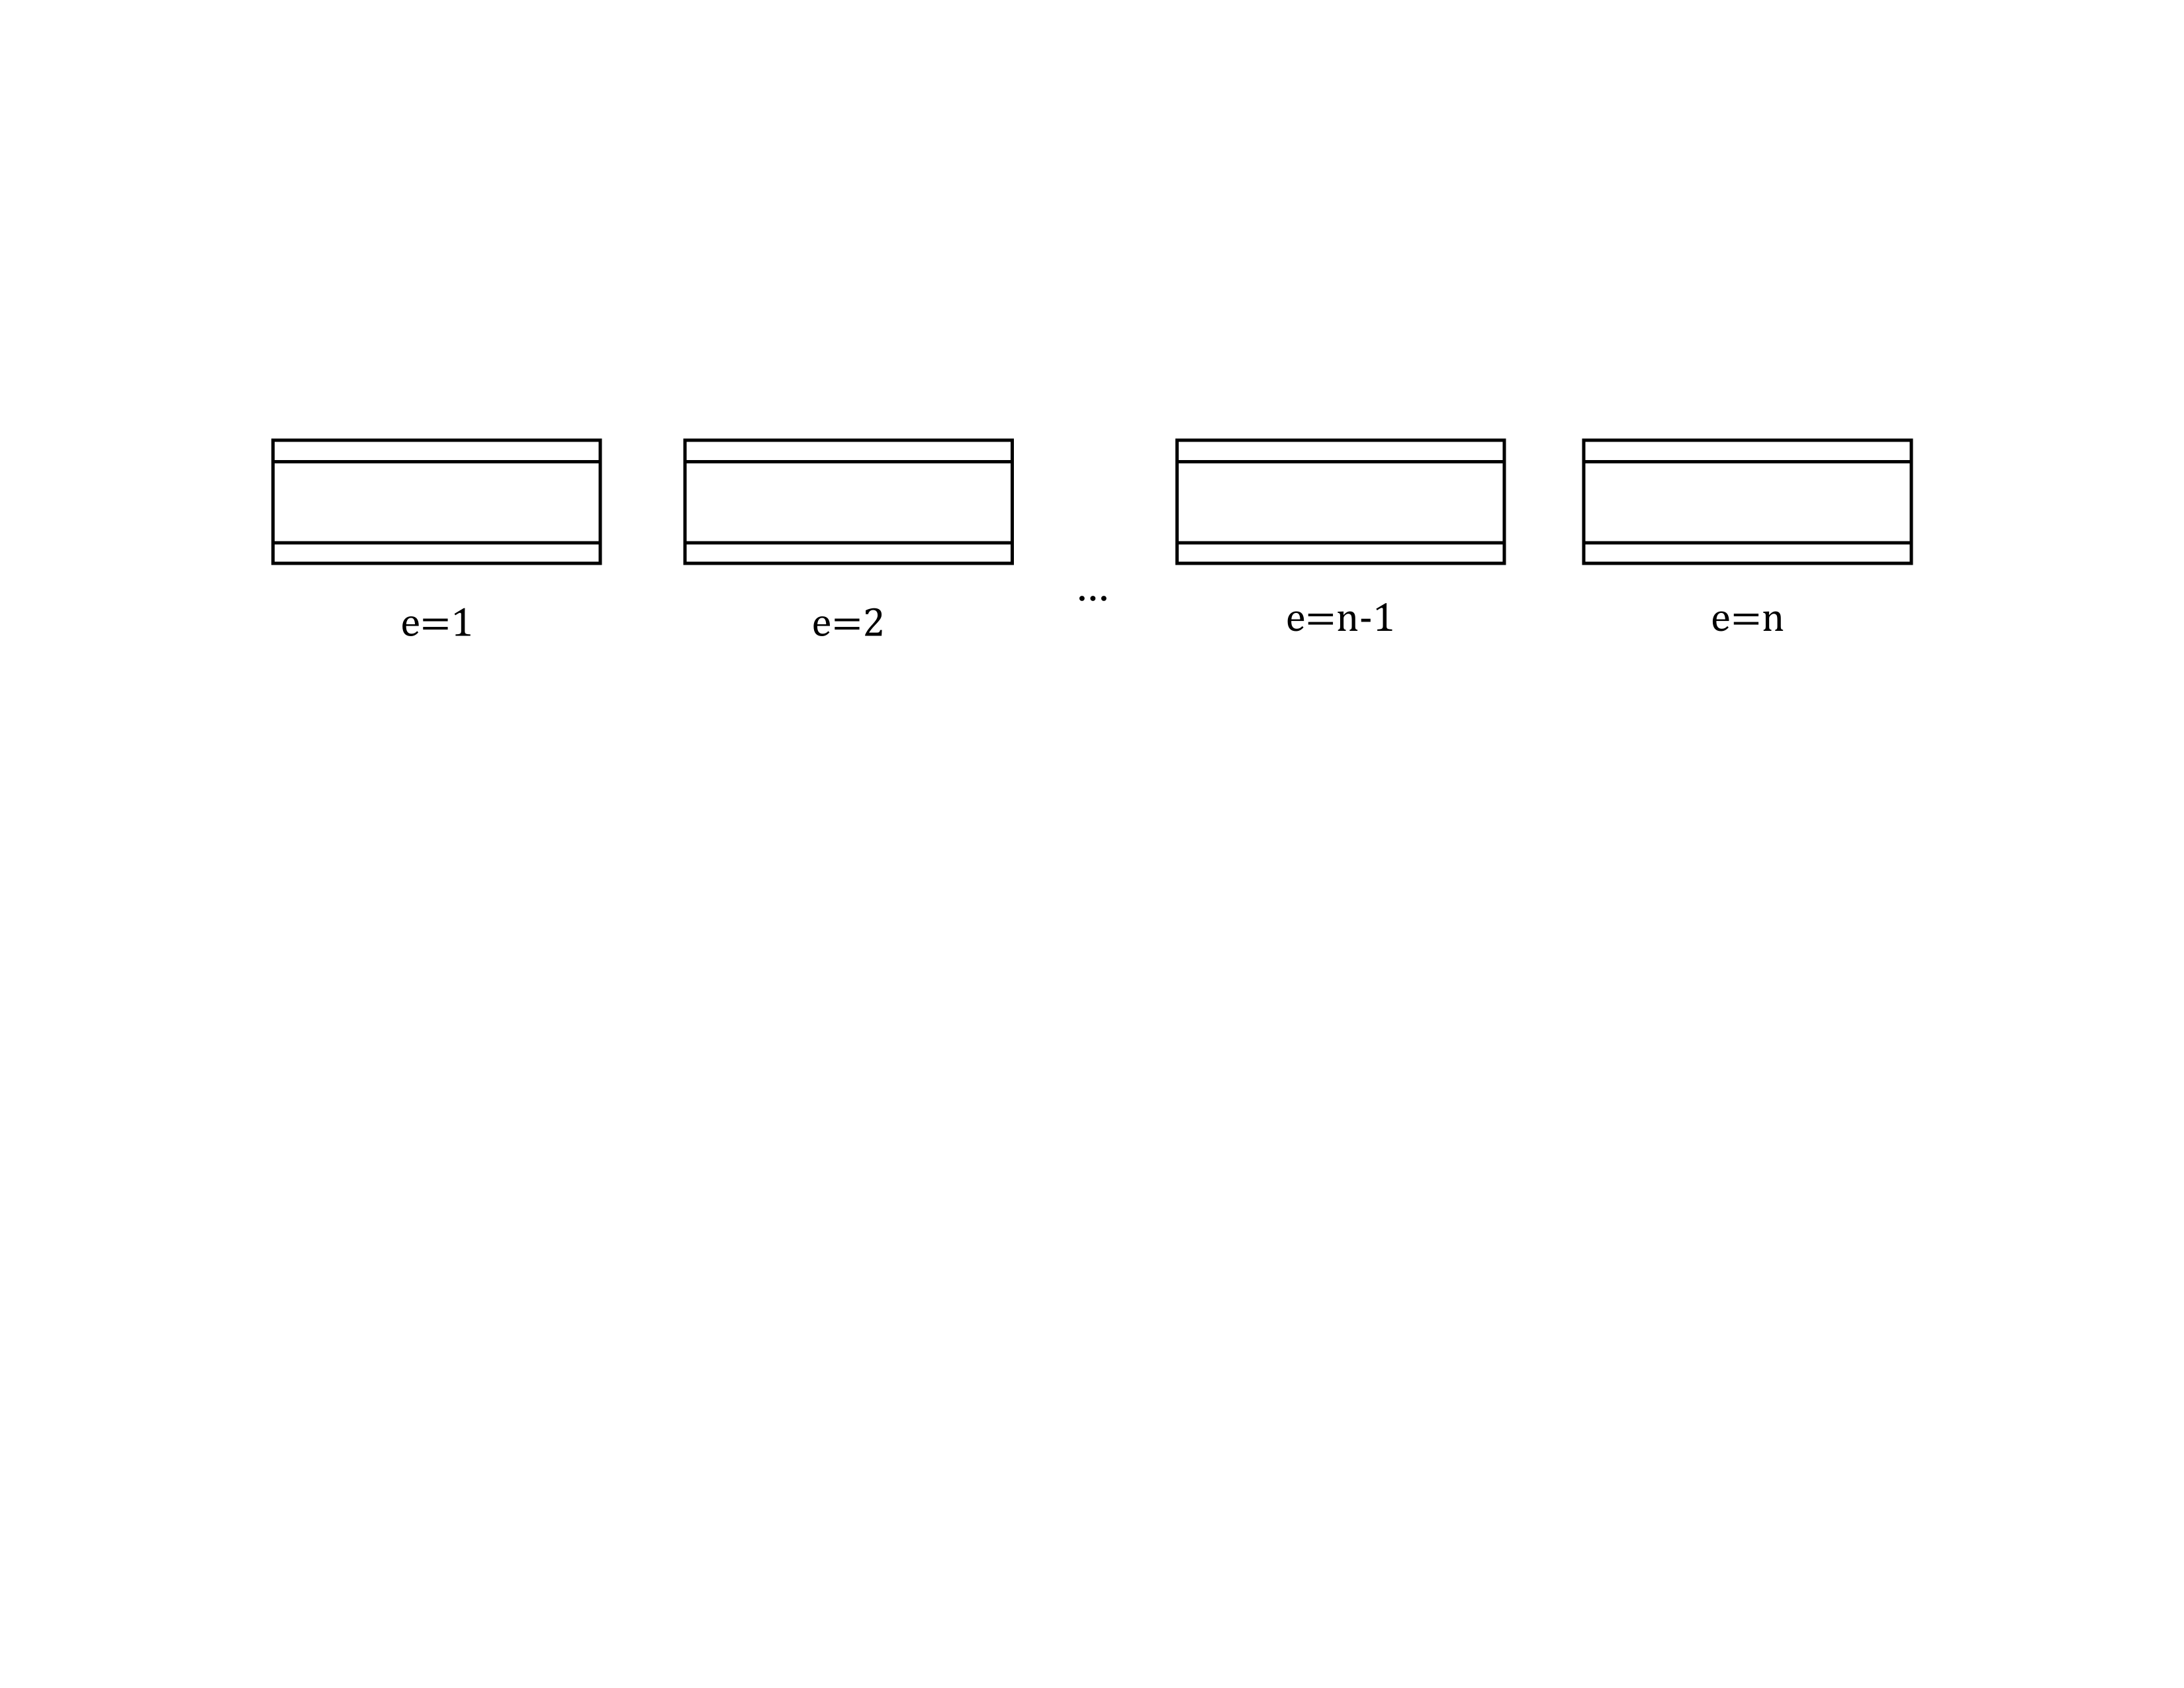
\includegraphics[width=0.7\columnwidth,trim=0cm 12cm 0cm 0cm, clip]{figs/wshape_elements.png}
\caption{The beam subdivided into n elements}
\label{fig:subdivision}
\end{figure}

\begin{figure}[htb]
\centering
\subfloat[side view]{
	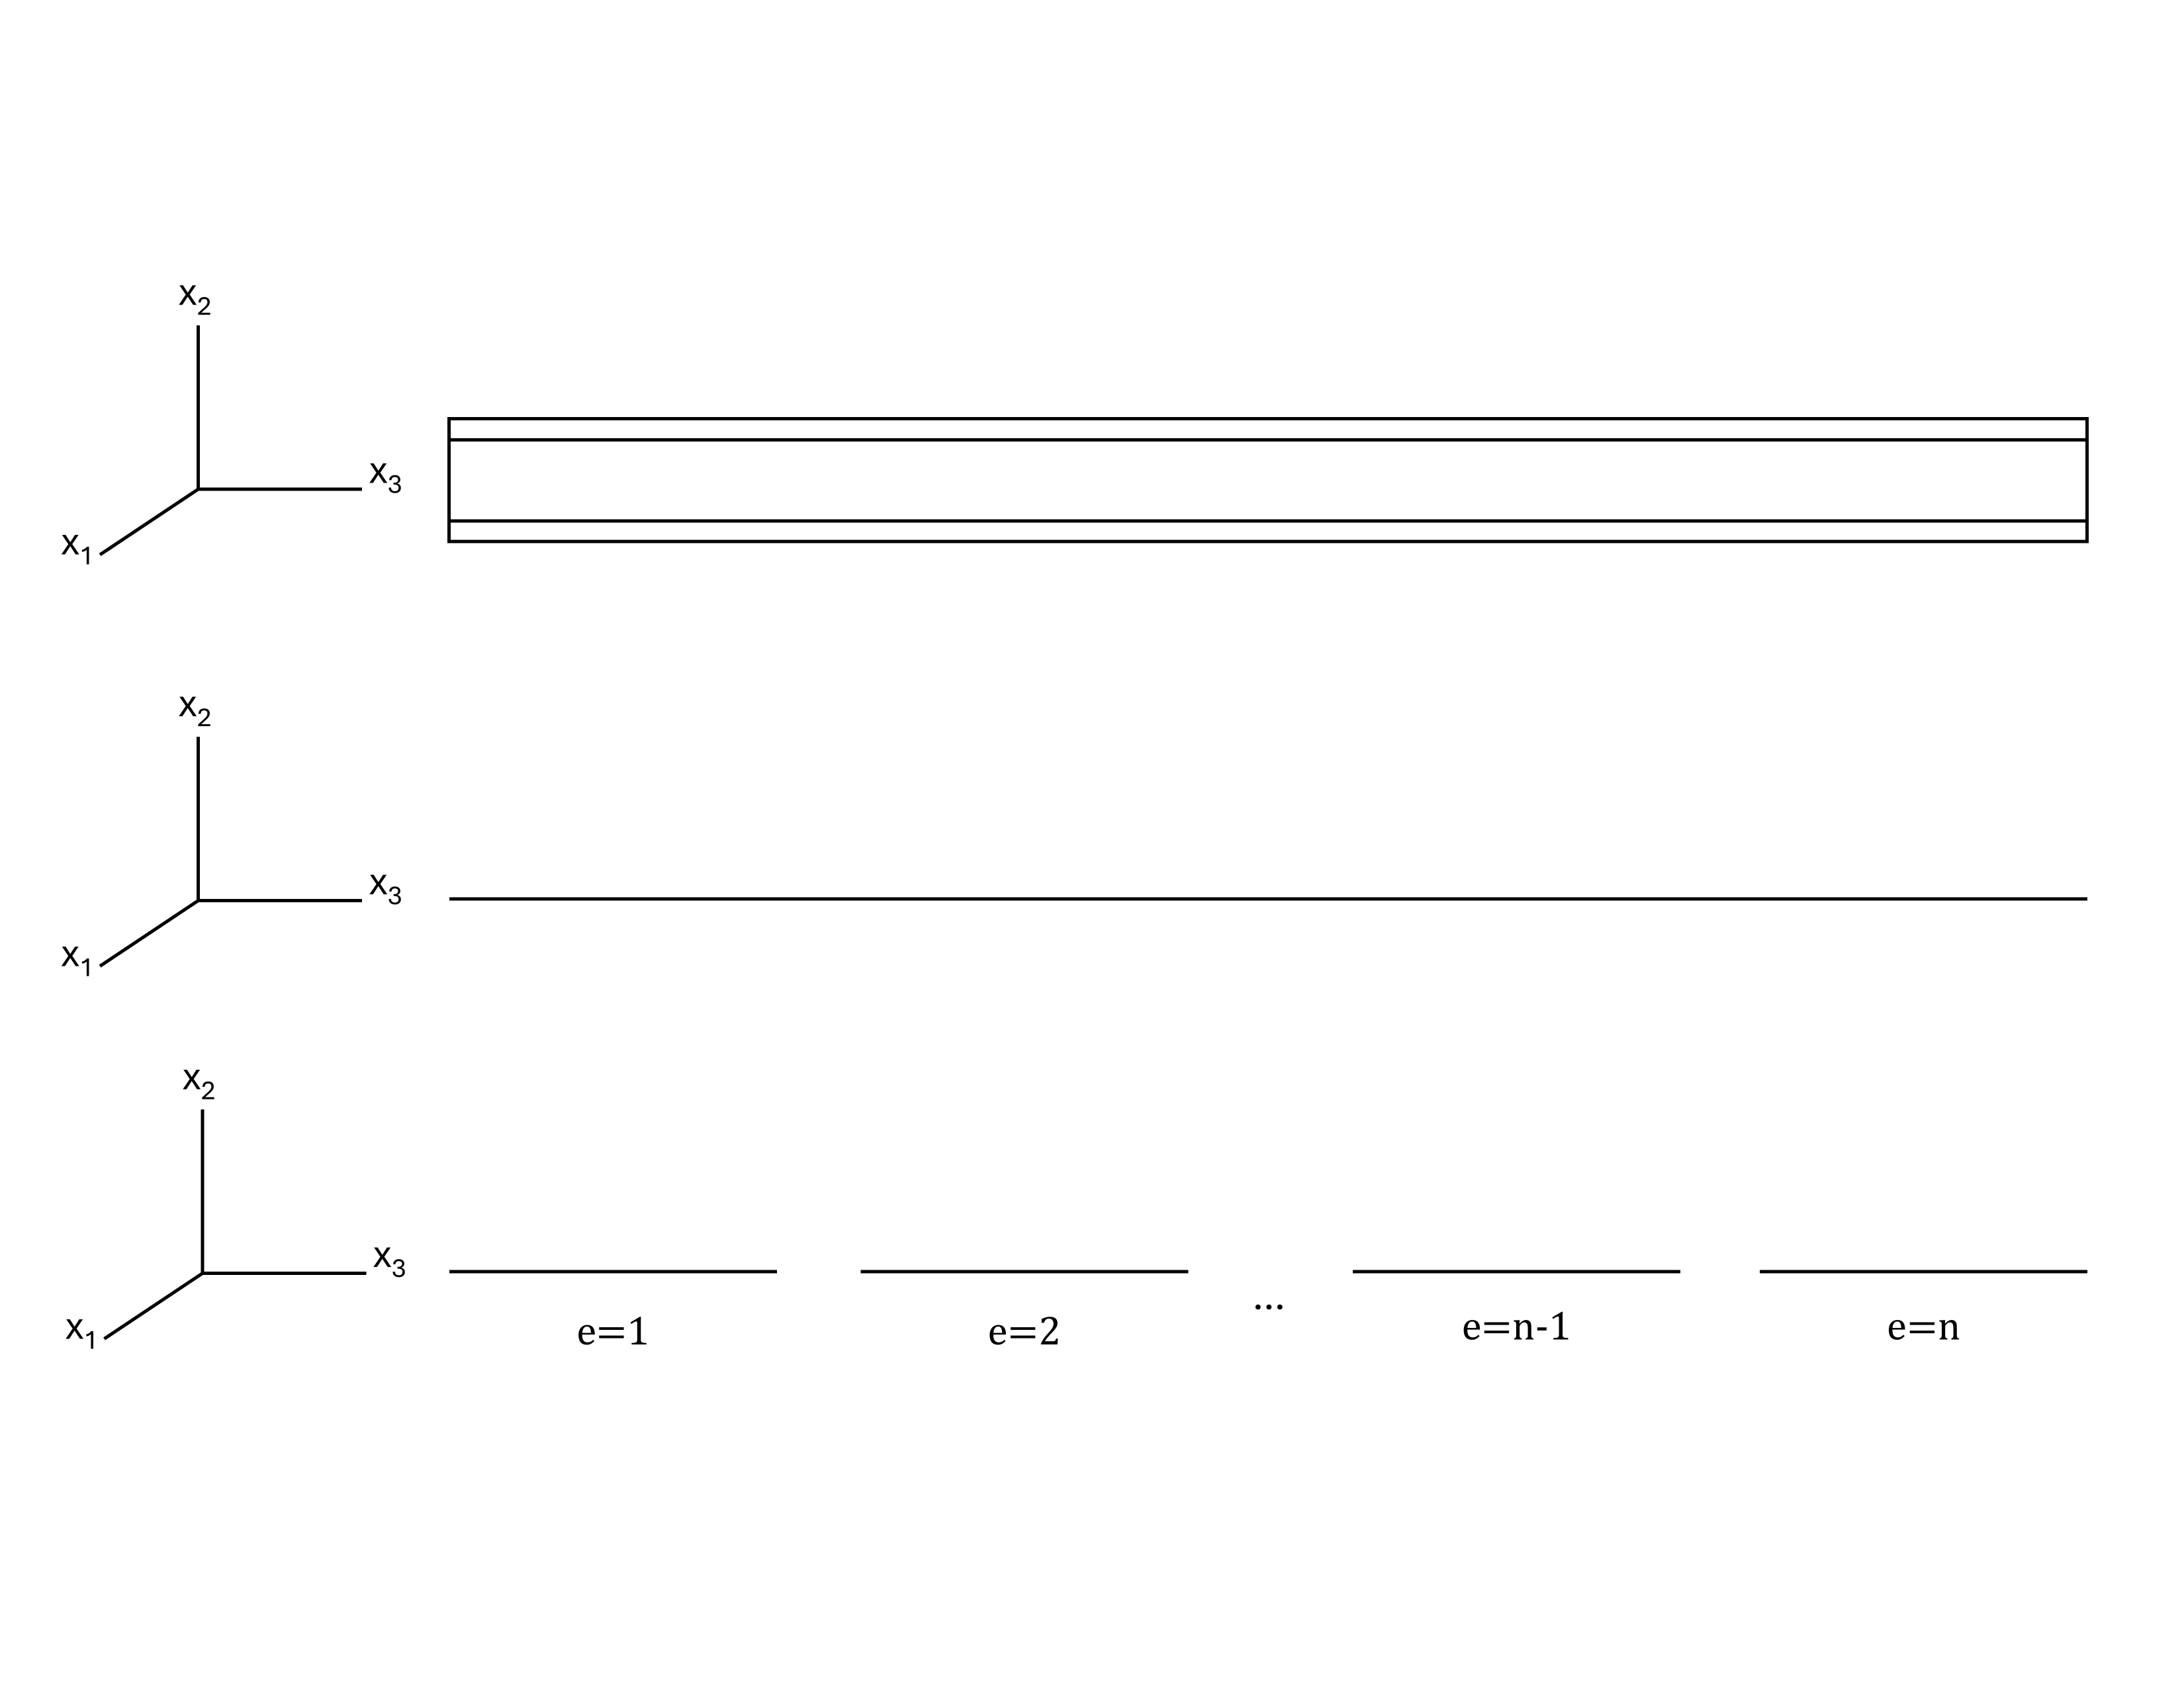
\includegraphics[width=0.7\columnwidth,trim=0cm 13cm 0cm 0cm, clip]{figs/beam_to_elements.png}
}
\centering
\subfloat[isometric view]{
	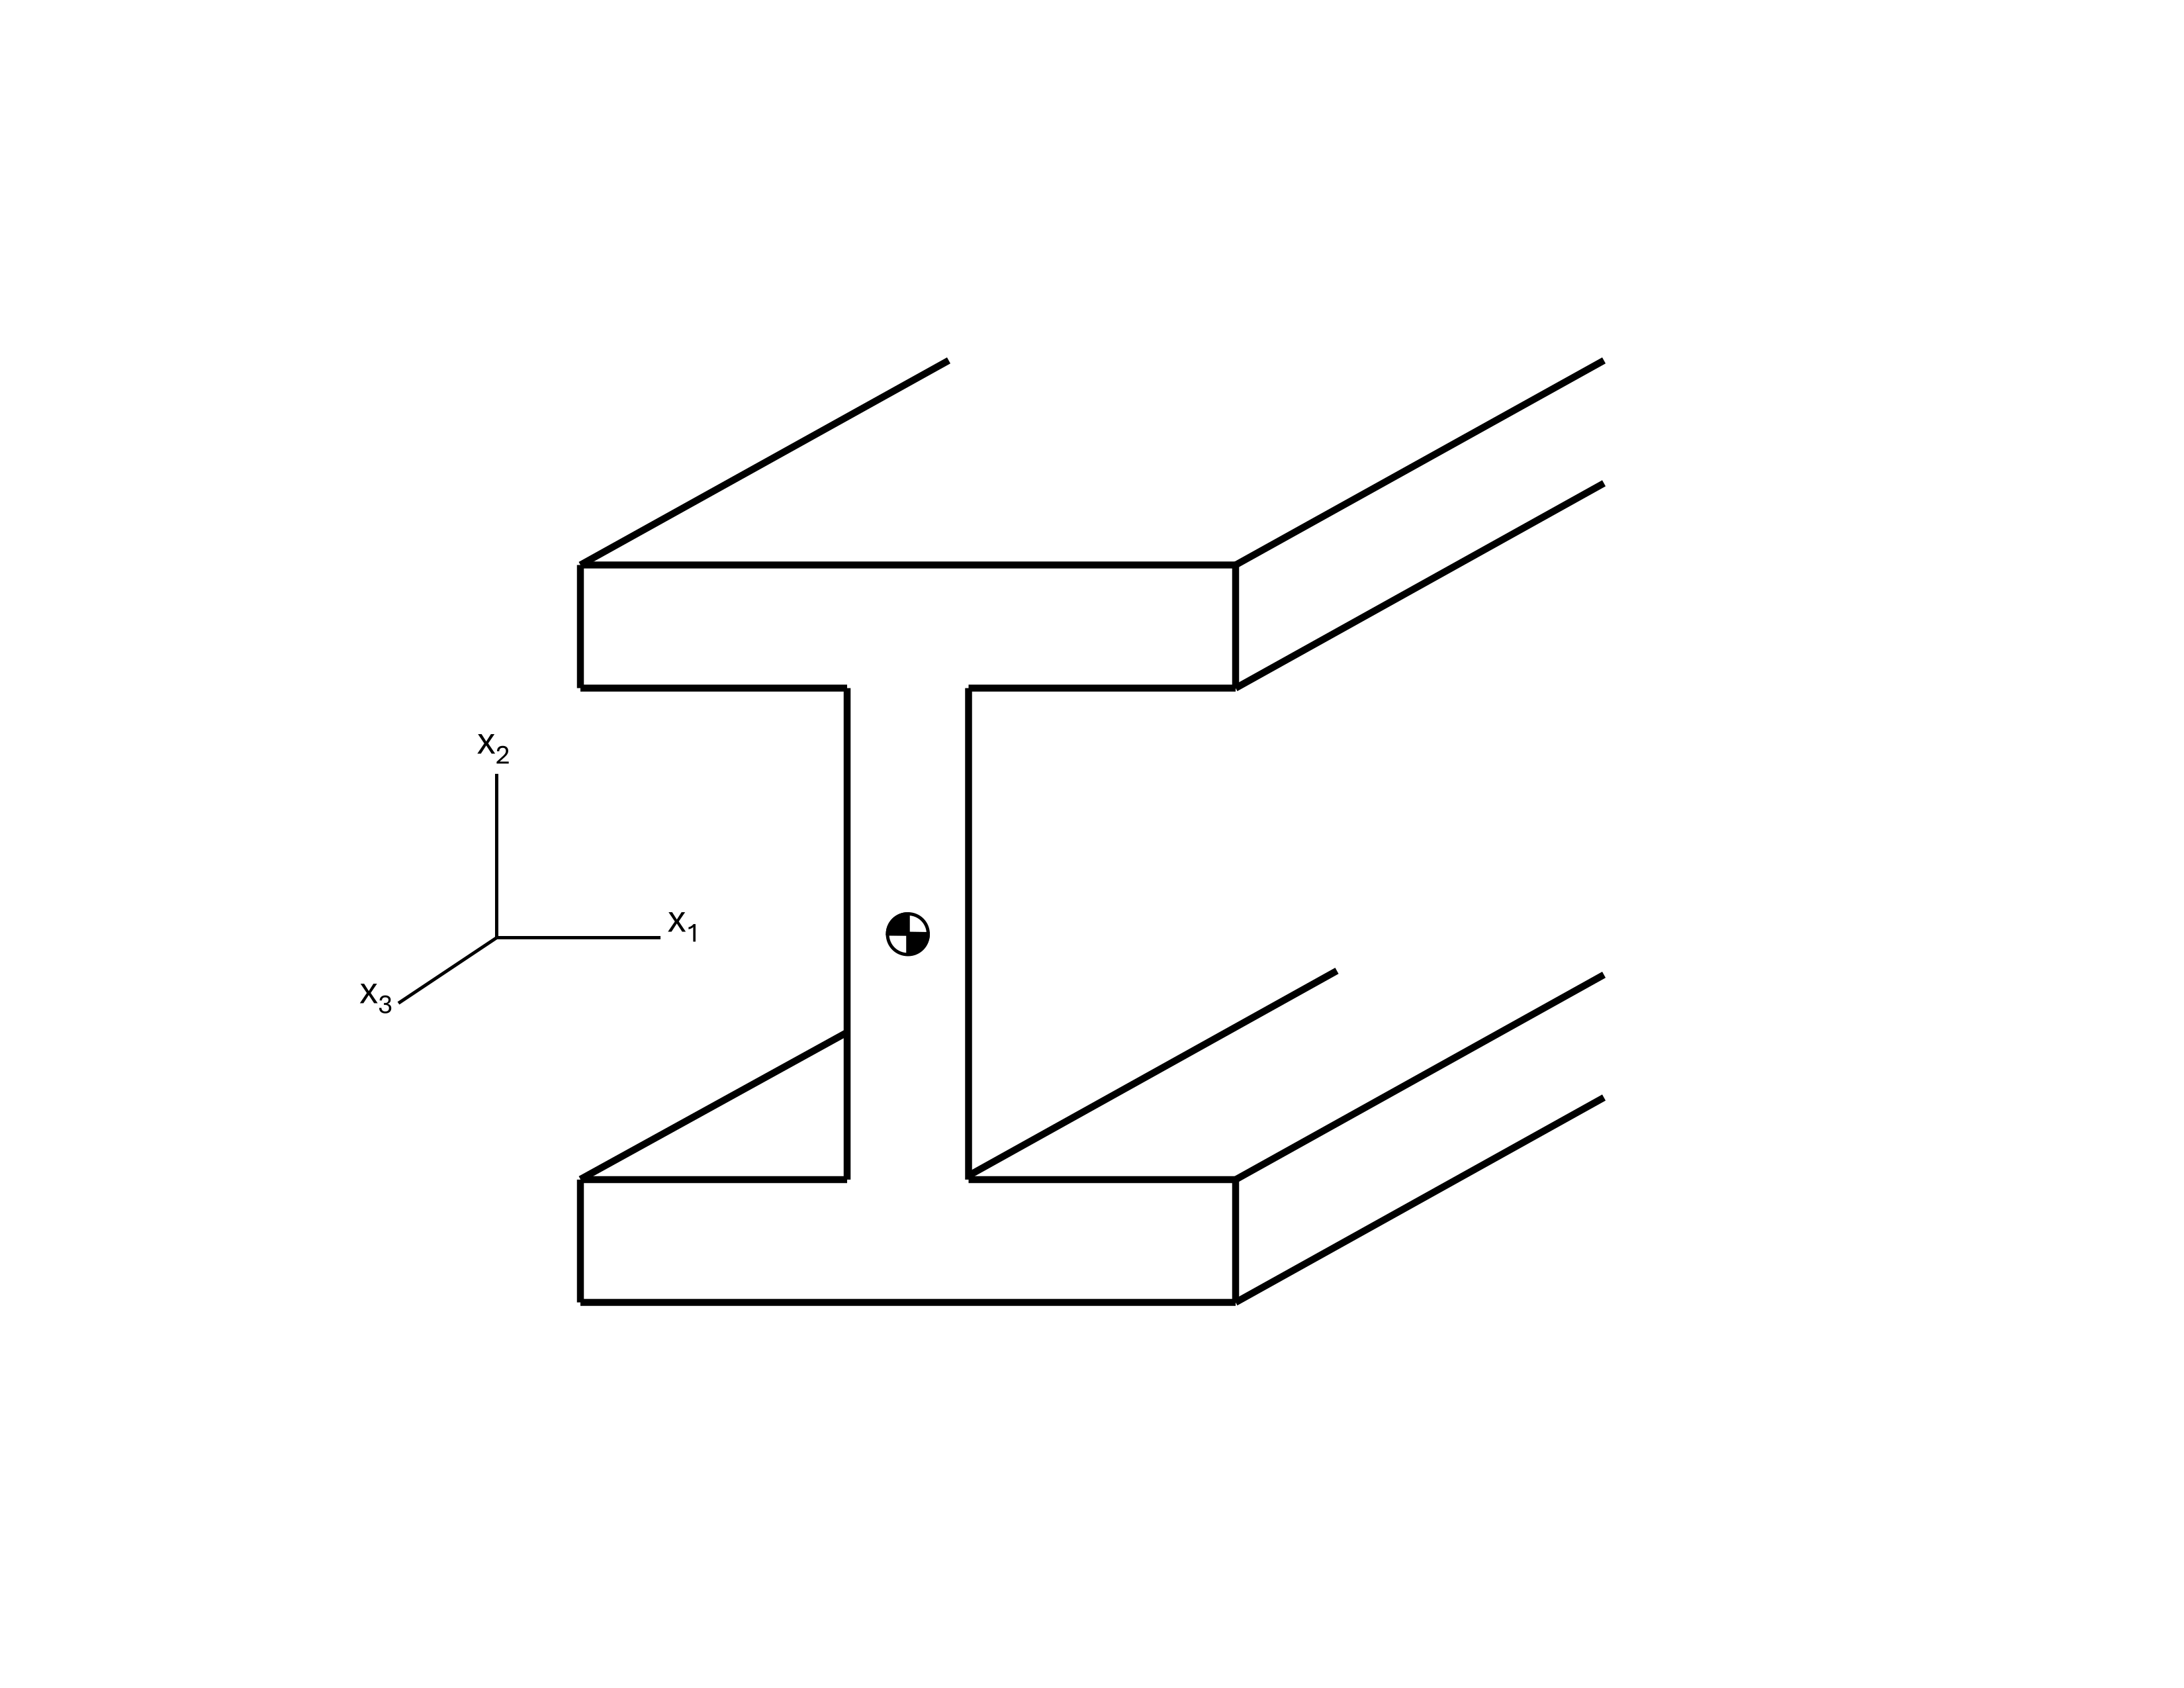
\includegraphics[width=0.25\columnwidth,trim=0cm 3cm 0cm 0cm, clip]{figs/3d_section.png}
	\label{fig:iso_view}
}
\caption{The definition of the beam}
 \label{fig:axis_definition}
\end{figure}

I will begin by outlining the assumptions made.

\paragraph{Approximating the Beam}
 We will first define a beam as our domain of interest.
The beam is displayed in \cref{fig:beam_definition}.
The domain of our beam is to first be divided into multiple sections, as shown in \cref{eq:subdivision} and \cref{fig:subdivision}, where 
$\Omega$ is the beam,
$\Omega^e$  is the $e$th element of the beam, and
$\overset{n}{\underset{e=1}{\cup}}$ is the union from element 1 to n.

\begin{equation}
 \Omega = \overset{n}{\underset{e=1}{\cup}} \Omega^e
 \label{eq:subdivision}
 \end{equation}


Thus \cref{eq:subdivision} states that the domain of interest is to be composed of beam elements numbered from 1 to n.
Furthermore, each element has local axes defined with respect to the principal axes as shown in \cref{eq:axis_definition,fig:axis_definition}, where $h^e$ is the length of each element and $A^e$ is the cross sectional area of each element.

\begin{equation}
\Omega^e = \{
(x_1^e, x_2^e, x_3^e)
|x_3^e 
\in 
[0,h^e], 
(x_1^e, x_2^2) 
\in
A^e 
\subset
\mathbb{R}^2 
\}
\label{eq:axis_definition}
\end{equation}

Furthermore, for the analysis the beam will be considered a one dimensional element. 
Thus, the beam will be approximated as a line with length $h$ that will act at the centroid of the beam as shown by the center of gravity marker in~\cref{fig:iso_view}.
In other texts, this is represented by~\cref{eq:zero_area}.

\begin{equation}
0 =
\int_{A^e} x_1^e \,dA \  =
\int_{A^e} x_2^e \,dA \ =
\int_{A^e} x_1^e x_2^e \,dA \
\label{eq:zero_area}
\end{equation}

\paragraph{Stress Tensor}
The second assummption is that $\sigma_{\alpha\beta}=0$ for $\alpha,\beta \in \{1,2\}$.
The stress tensor $\sigma$ is shown in \cref{eq:stress_tensor} and the stress element in \cref{fig:stress_element}.
By this assumption, the beam will not have normal stresses in the $x_1$ or $x_2$ directions, similar to an axial rod.
The difference between the beam and an axial rod is that it can experience shear in the $\sigma_{13}$ and $\sigma_{23}$ directions).
We know the beam will have loads applied in the $x_1$ or $x_2$ directions, which typically would mean a normal stress in those directions.
However, given our assumptions the beam will still be able to support these loads by the shear.
This assumption is made for consistency to ensure $\epsilon_{\alpha\beta} = 0$, since we are also neglecting the cross-sectional area of the beam as was shown in \cref{eq:zero_area}.
In \cref{sec:continuum_mechanics} it will be explained how we can still calculate $\epsilon_{\alpha\beta}$.

\begin{equation}
\sigma = \begin{bmatrix}
0 & 0 & \sigma_{13} \\
0 & 0 & \sigma_{23} \\
\sigma_{13} & \sigma_{23} & \sigma_{33}
\end{bmatrix}
\label{eq:stress_tensor}
\end{equation}

\begin{figure}%[htb]
\centering
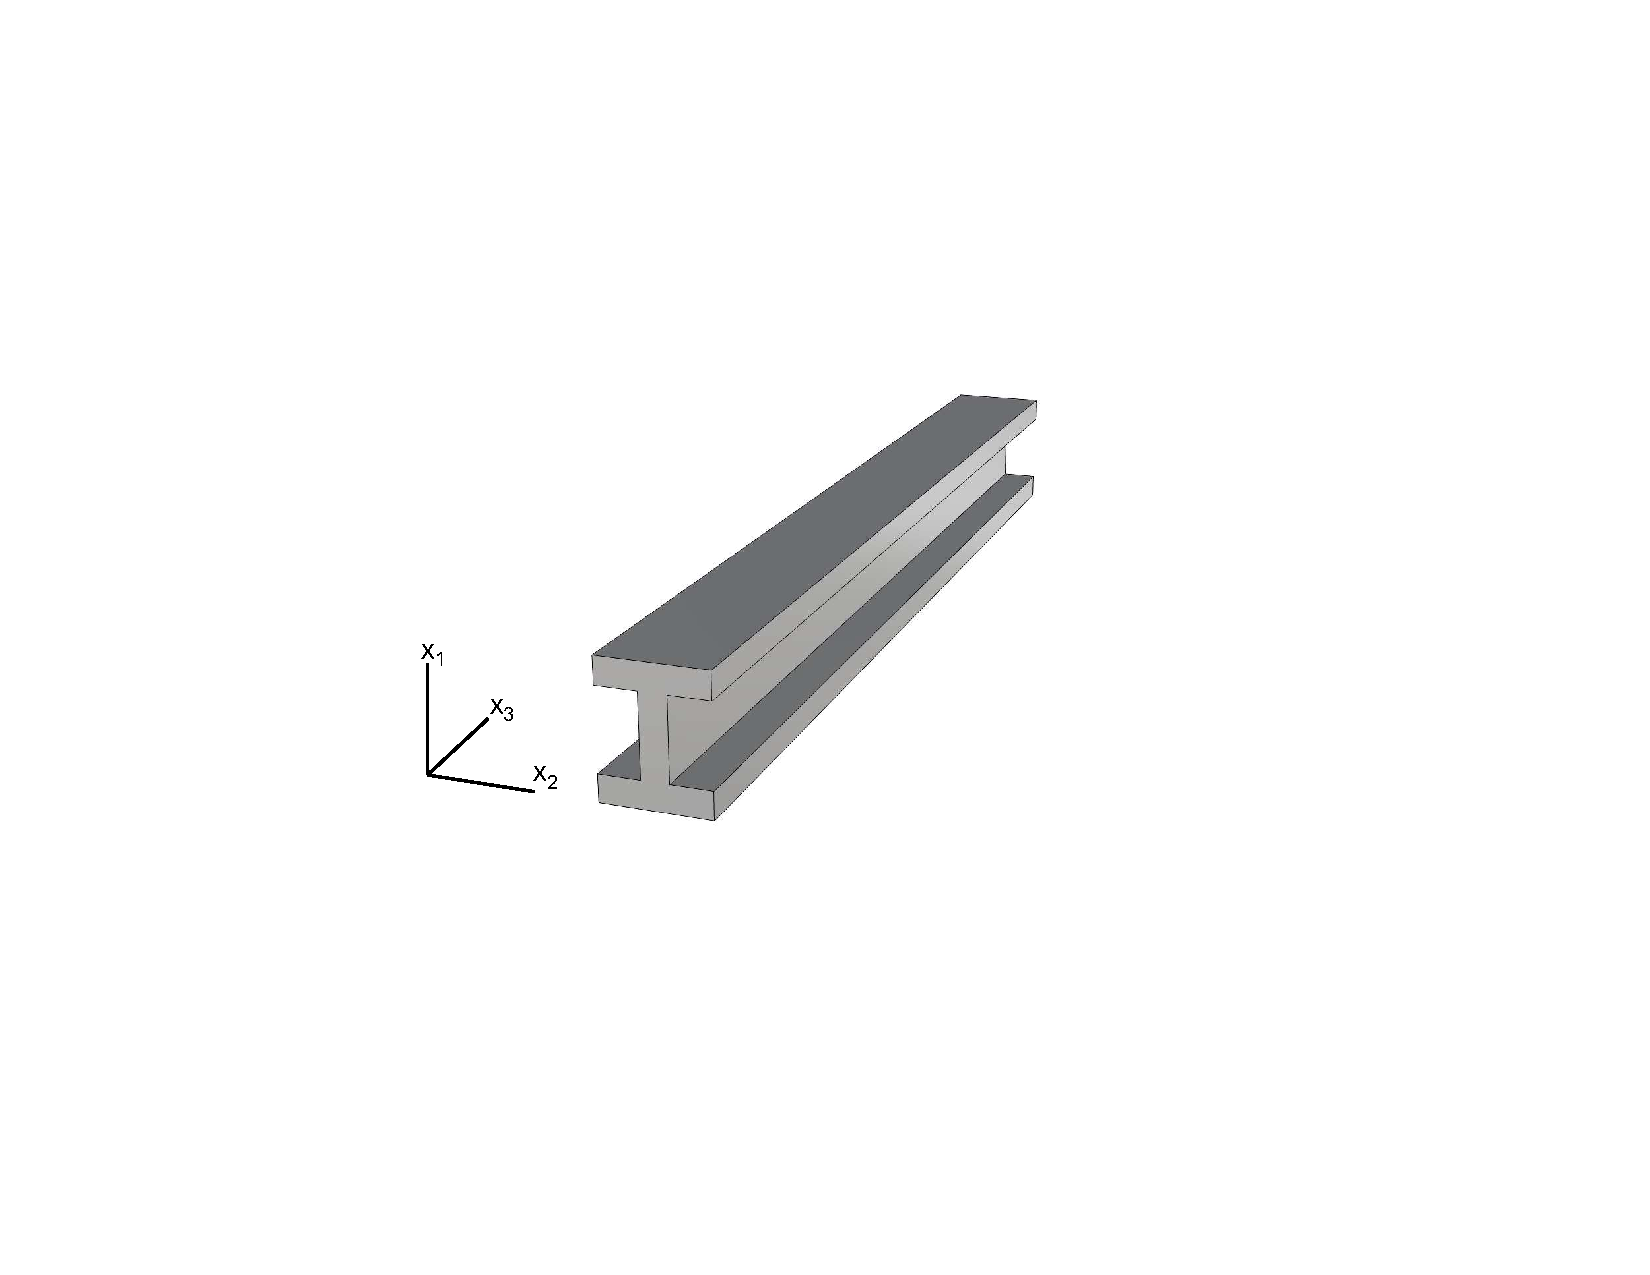
\includegraphics[width=0.95\columnwidth,trim=4cm 7cm 6cm 6.5cm, clip]{figs/straight.pdf}
\caption{The stress element of the beam in its global coordinates. CHANGE PICTURE: make a stress element with coordinate axes shown.}
\label{fig:stress_element}
\end{figure}

If we transform $\sigma$ into its principal stress form we get \cref{eq:plane_stress_tensor}.
This is significant becasue it shows that the beam is in a plane stress condition. 
A general Mohr's circle for this state of stress is shown in \cref{fig:mohrs_circle}.
This seems to justify the fact that in mechanics of materials almost all the stress tensors we worked with were simplified to the plane stress condition or similar. 

\begin{equation}
\sigma* = \begin{bmatrix}
 \frac{\sigma_{33} + \sqrt{\sigma_{33}^2 + 4(\sigma_{13}^2 + \sigma_{23}^2)}}{2} & 0 & 0 \\
0 &  \frac{\sigma_{33} - \sqrt{\sigma_{33}^2 + 4(\sigma_{13}^2 + \sigma_{23}^2)}}{2} & 0 \\
0 & 0 & 0
\end{bmatrix}
\label{eq:plane_stress_tensor}
\end{equation}

\begin{figure}
\centering
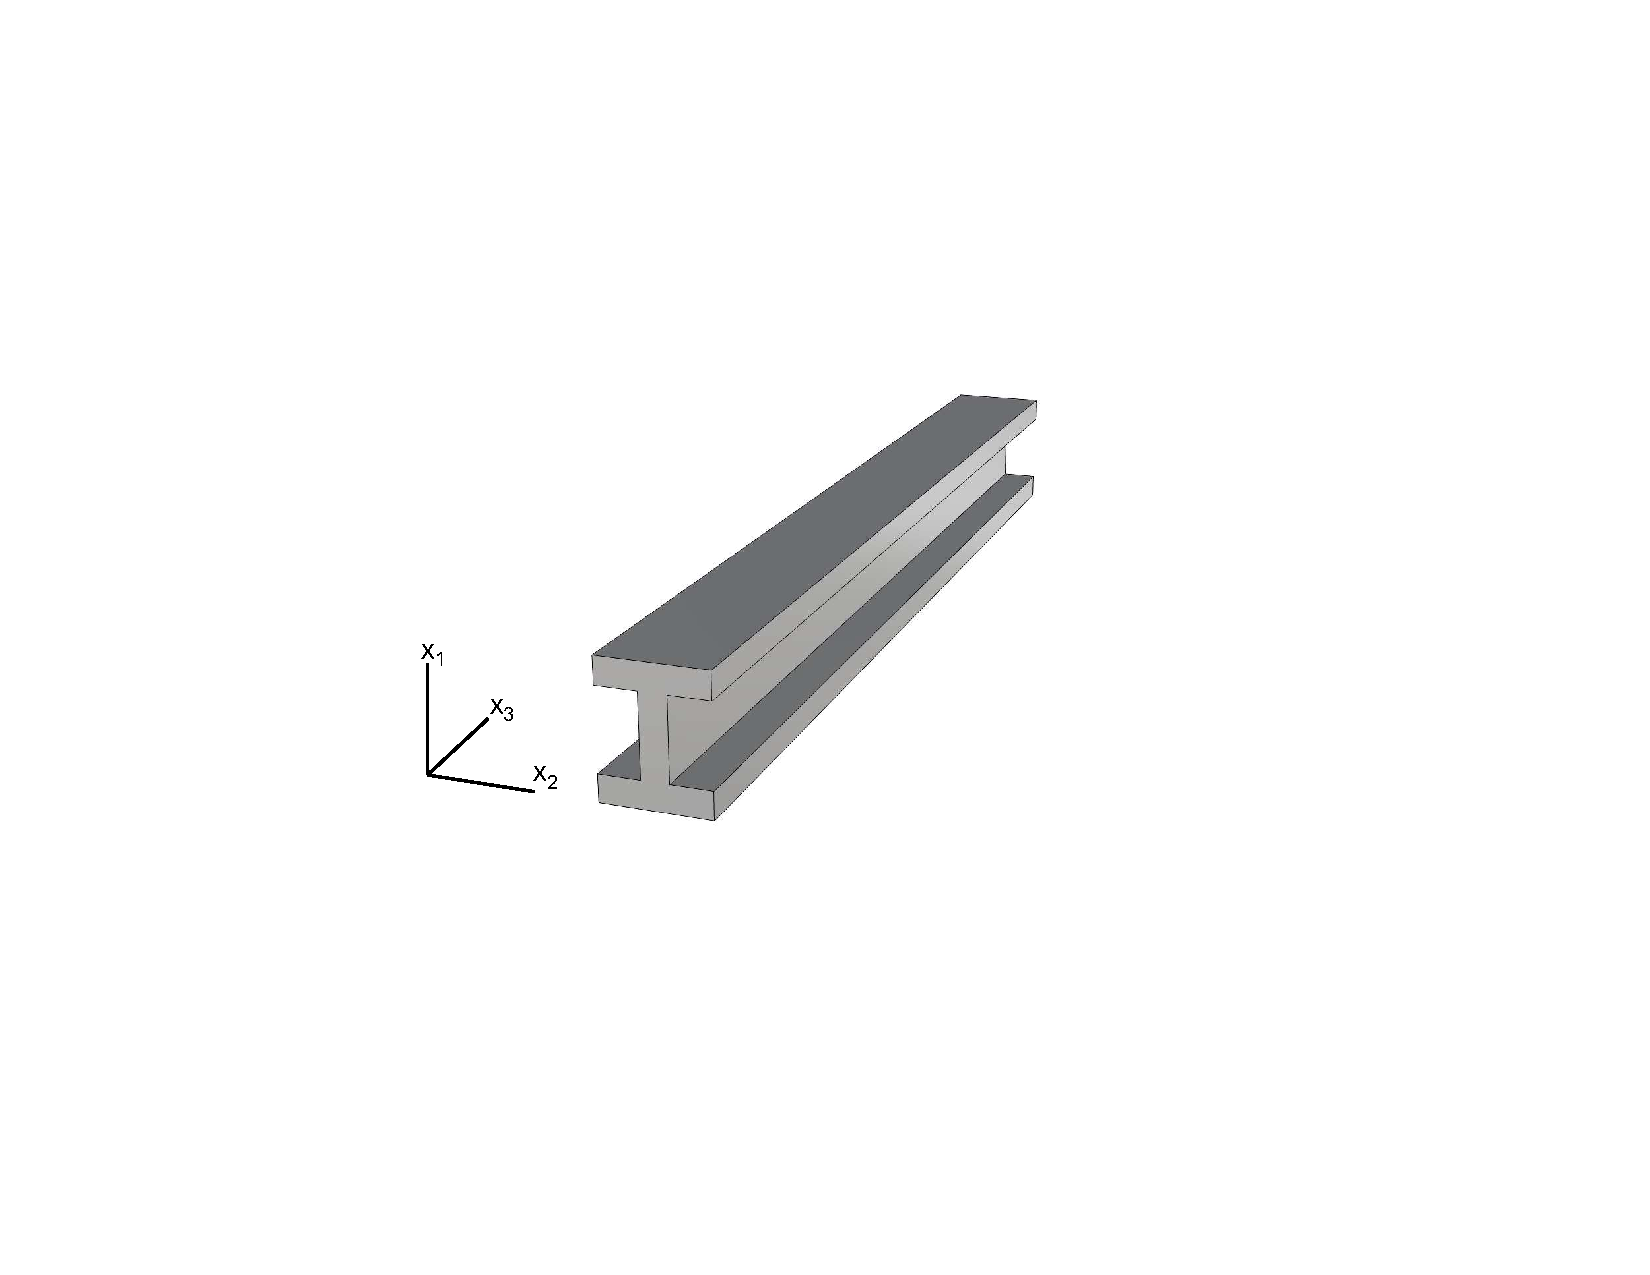
\includegraphics[width=0.95\columnwidth,trim=4cm 7cm 6cm 6.5cm, clip]{figs/straight.pdf}
\label{fig:mohrs_circle}
\caption{The generalized Mohr's circle for the plane stress condition. CHANGE PICTURE: make a Mohr's circle like the one on pg 85 (pg 25 of 61-80) in Continuum Mechanics Text}
\end{figure}

\paragraph{Displacements}
The kinematics of the beam will be accounted for using \cref{eq:u1, eq:u2, eq:u3}.
The translation of the beam is represented by $w_i$, where $i$ is the direction of the translation.
The rotation of the beam is represented by $\theta_i$.
As can be observed from the equations, $w_i$ and $\theta_i$ are functions of only $x_3$, the location along the length of the beam.
That is true because the beam is collapsed to a one-dimensional element.
The overall displacement of a point on the beam is $u_i$, which acts as a function of $x_1$, $x_2$, and $x_3$.
\cref{fig:w_theta_displacements} displays a positive displacement in each coordinate direction for both translations and rotations. 

\begin{equation}
u_1(x_1, x_2, x_3)=w_1(x_3)-x_2\theta_3(x_3)
\label{eq:u1}
\end{equation}

\begin{equation}
u_2(x_1, x_2, x_3)=w_2(x_3)+x_1\theta_3(x_3)
\label{eq:u2}
\end{equation}

\begin{equation}
u_3(x_1, x_2, x_3)=w_3(x_3)-x_1\theta_2(x_3)+x_2\theta_1(x_3)
\label{eq:u3}
\end{equation}

\begin{figure}
\centering
\subfloat[No displacement]{
	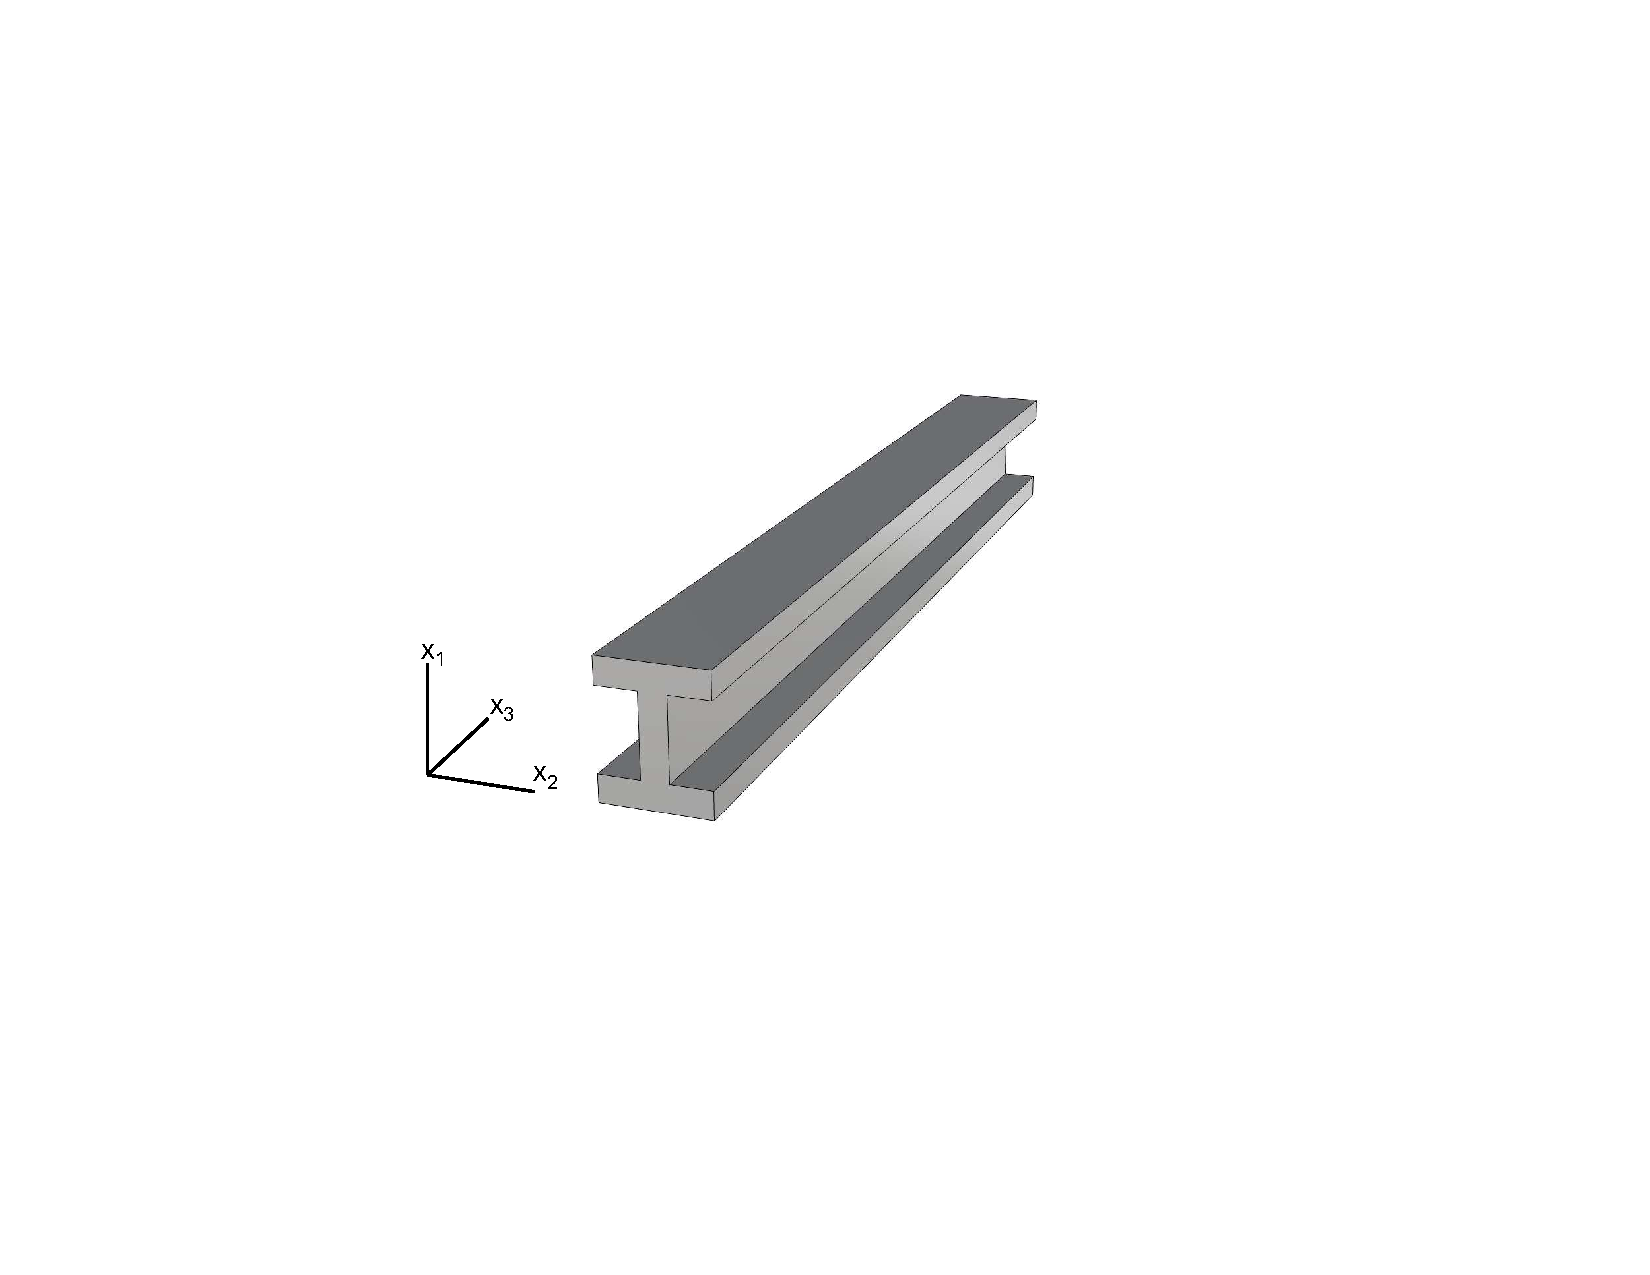
\includegraphics[width=0.2\columnwidth,trim=4cm 7cm 6cm 6.5cm, clip]{figs/straight.pdf}
}
\\
\subfloat[$w_1$]{
	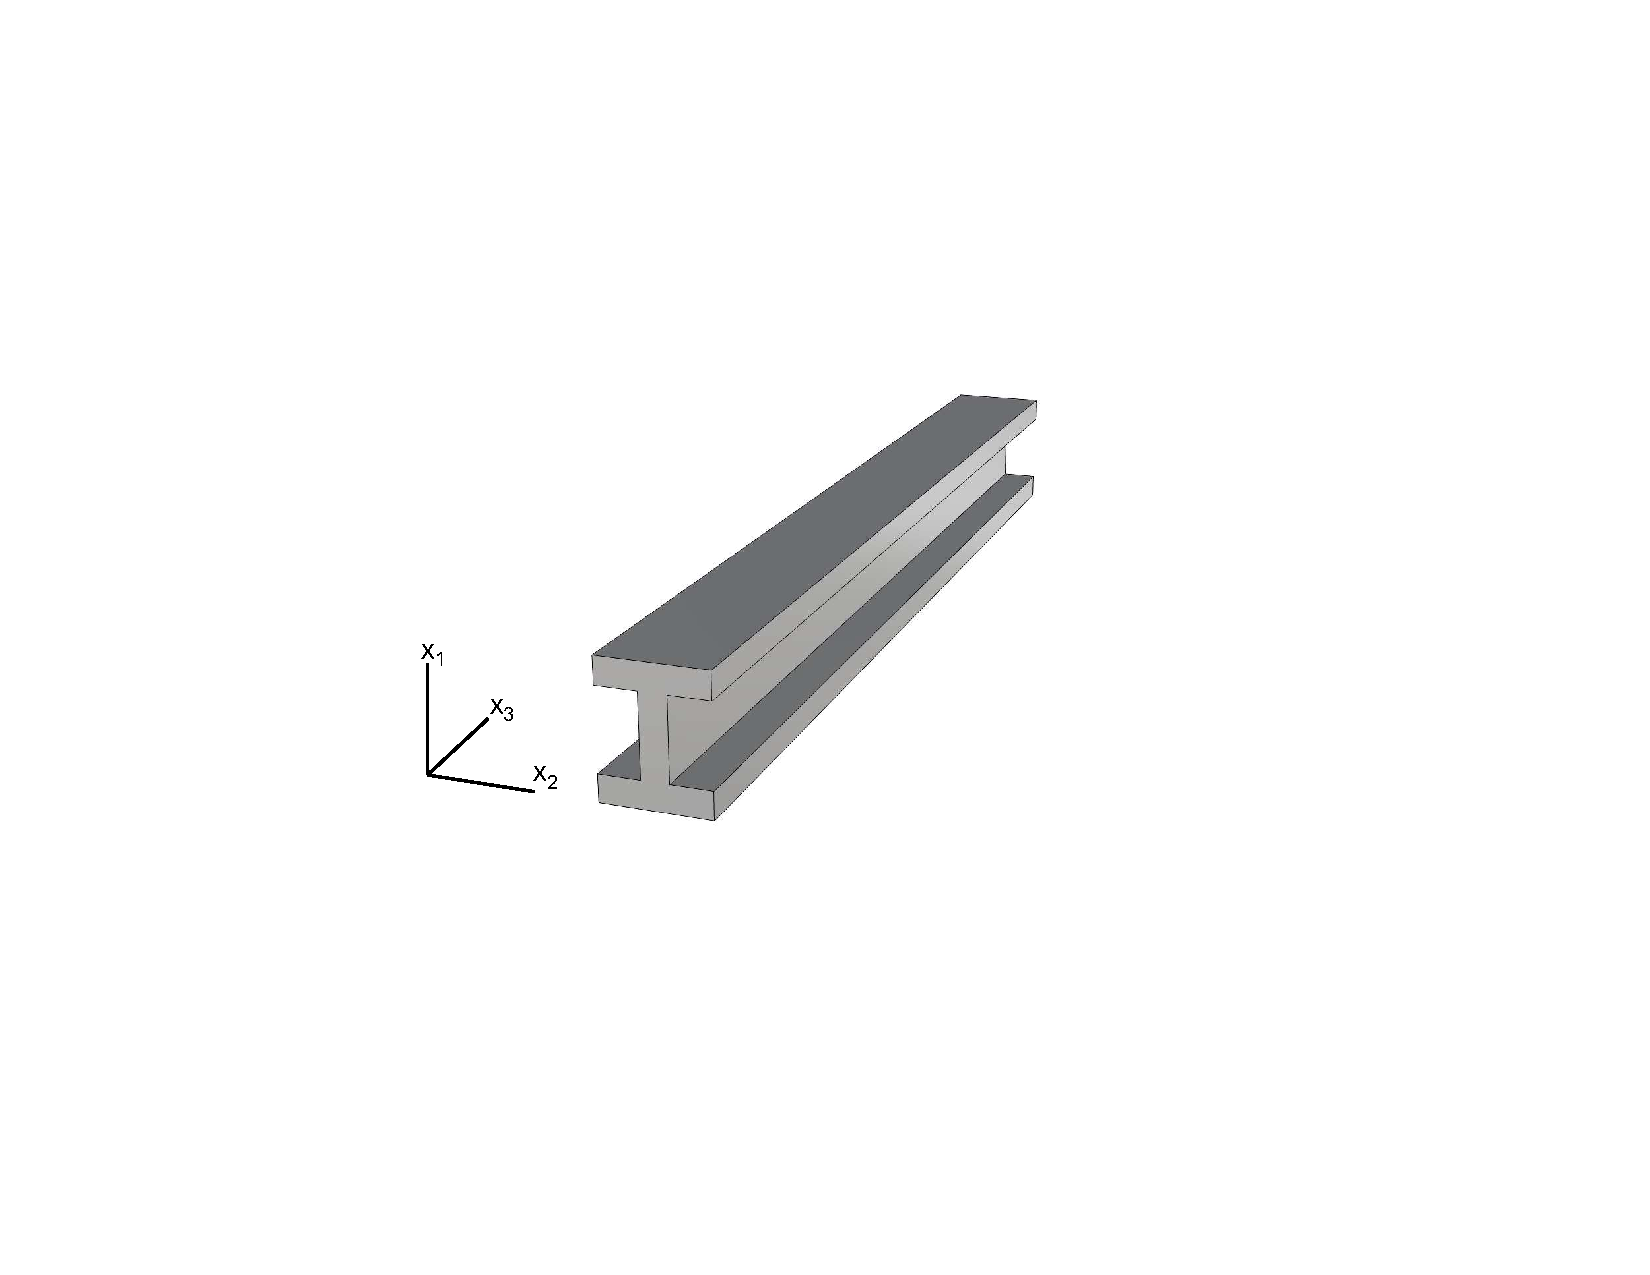
\includegraphics[width=0.2\columnwidth,trim=4cm 7cm 6cm 6.5cm, clip]{figs/straight.pdf}
}
\subfloat[$w_2$]{
	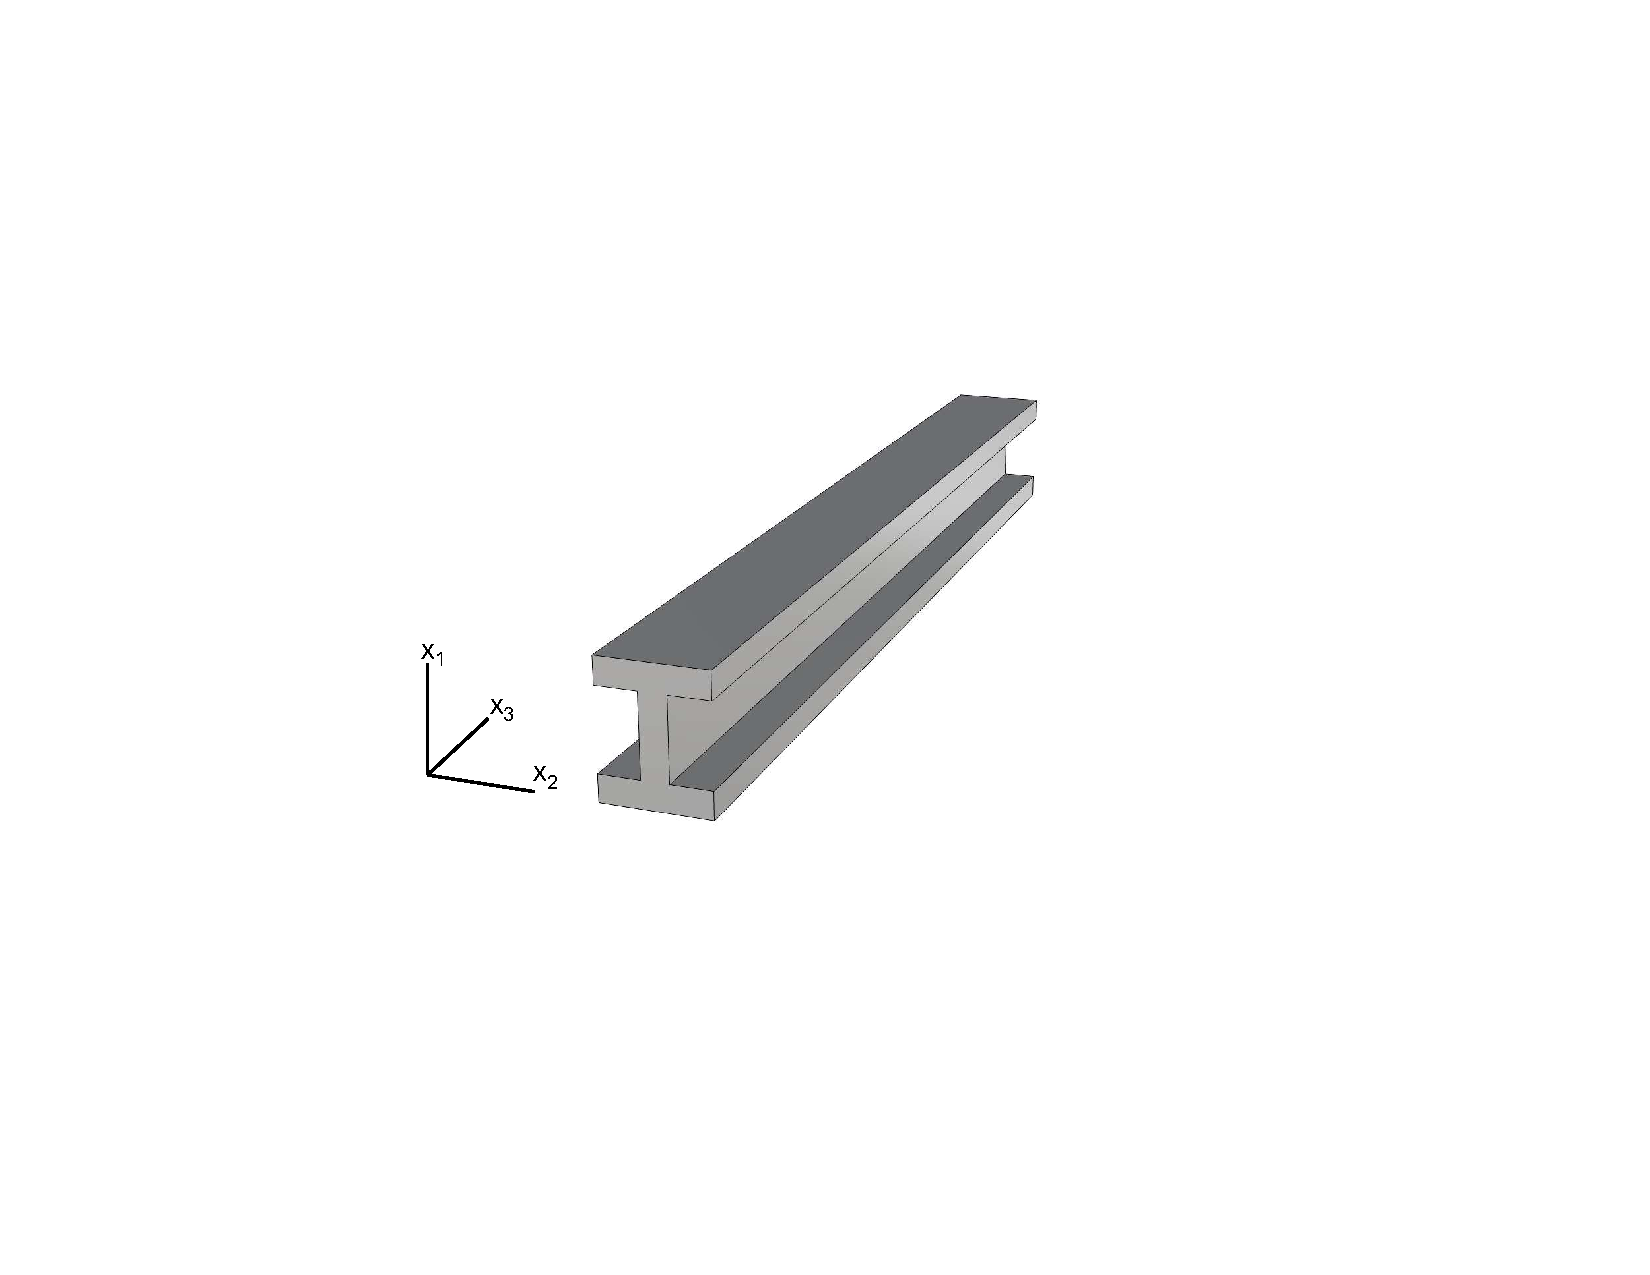
\includegraphics[width=0.2\columnwidth,trim=4cm 7cm 6cm 6.5cm, clip]{figs/straight.pdf}
}
\subfloat[$w_3$]{
	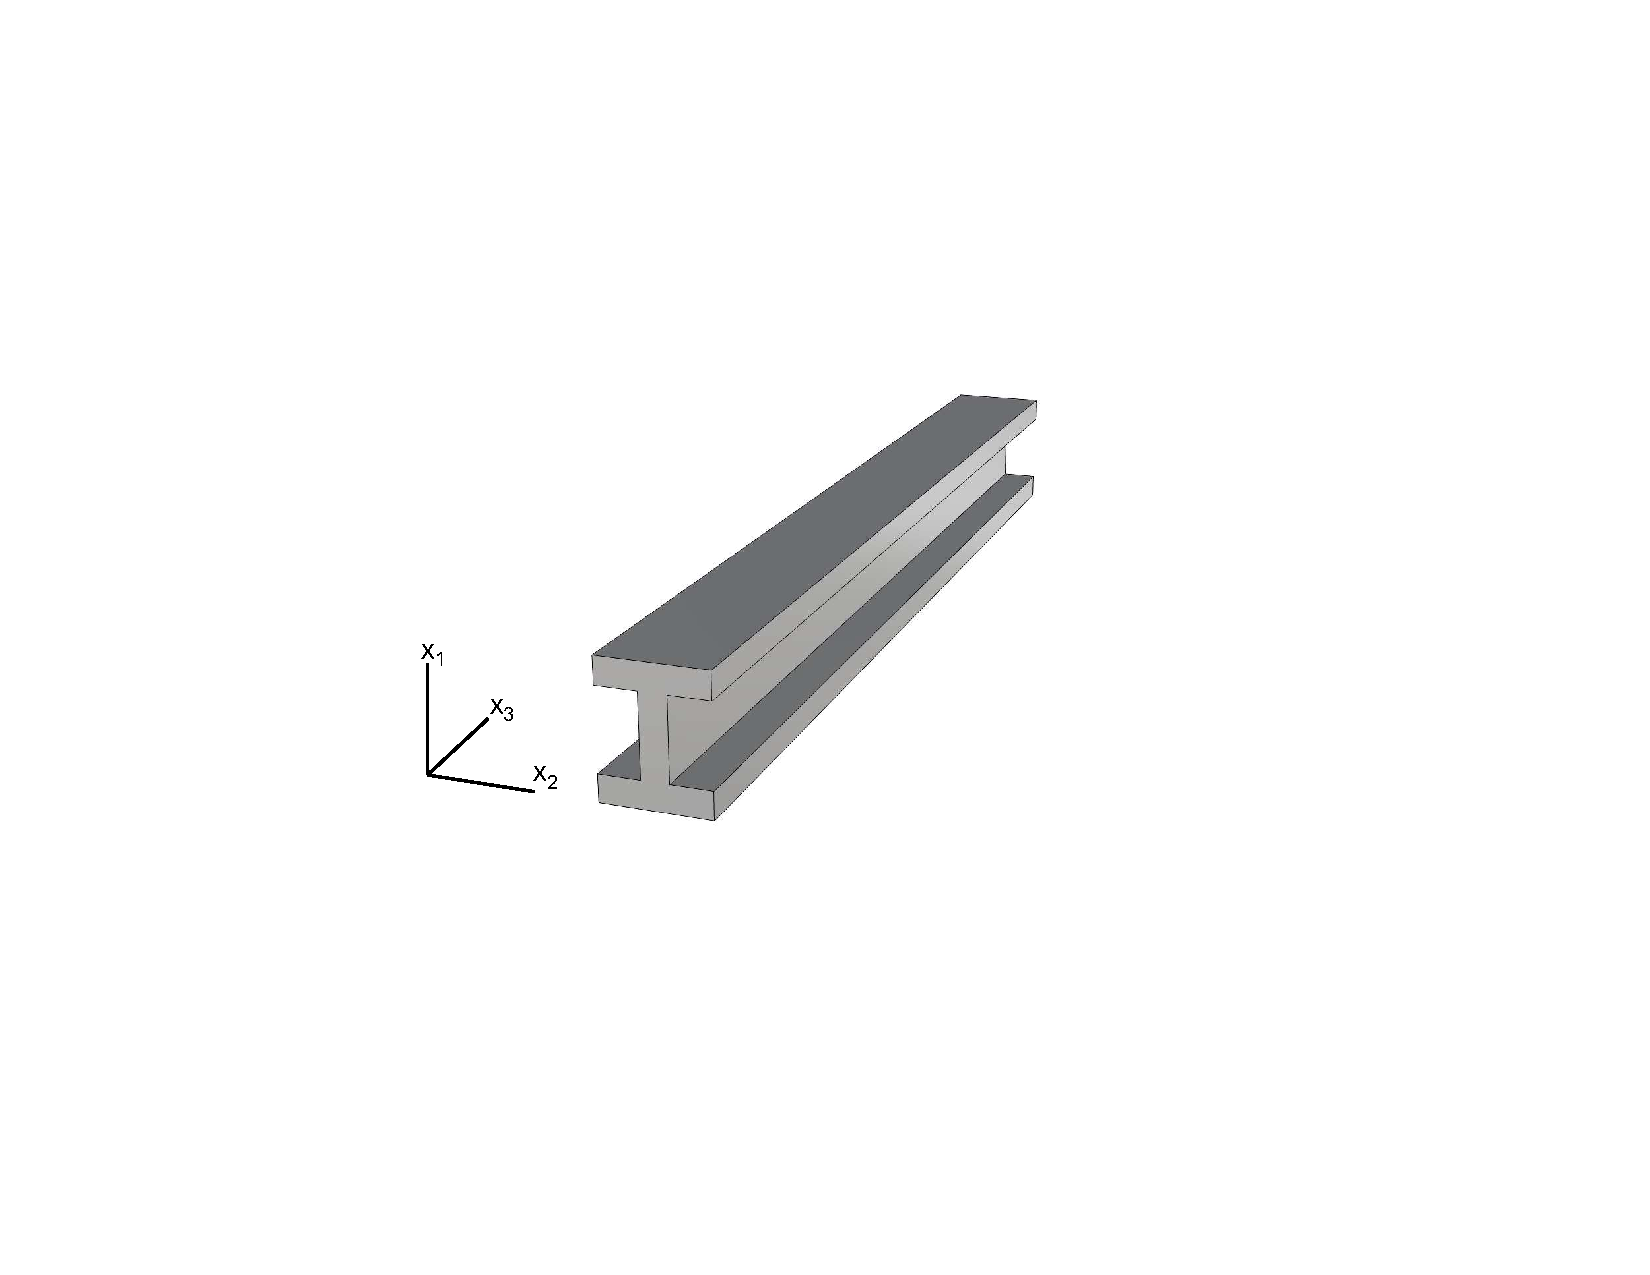
\includegraphics[width=0.2\columnwidth,trim=4cm 7cm 6cm 6.5cm, clip]{figs/straight.pdf}
}
\\
\subfloat[$\theta_1$]{
	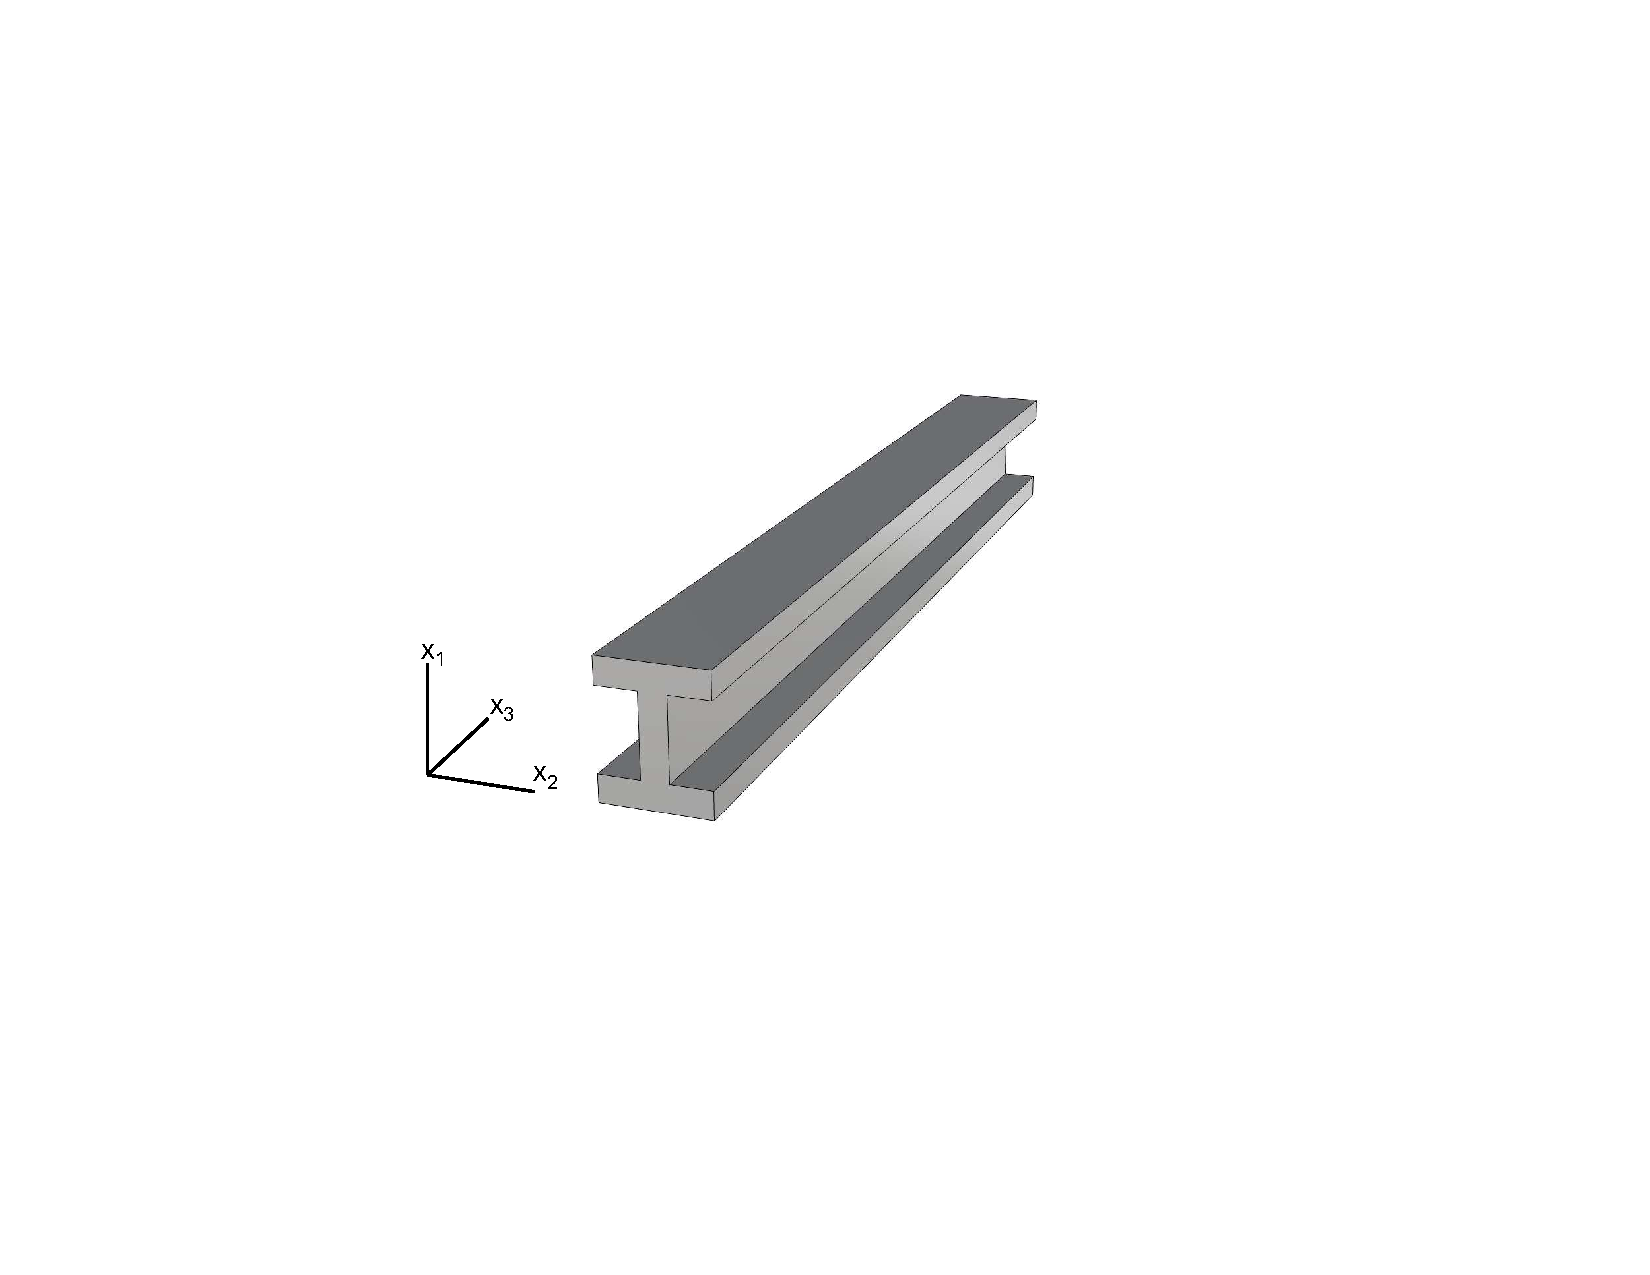
\includegraphics[width=0.2\columnwidth,trim=4cm 7cm 6cm 6.5cm, clip]{figs/straight.pdf}
}
\subfloat[$\theta_2$]{
	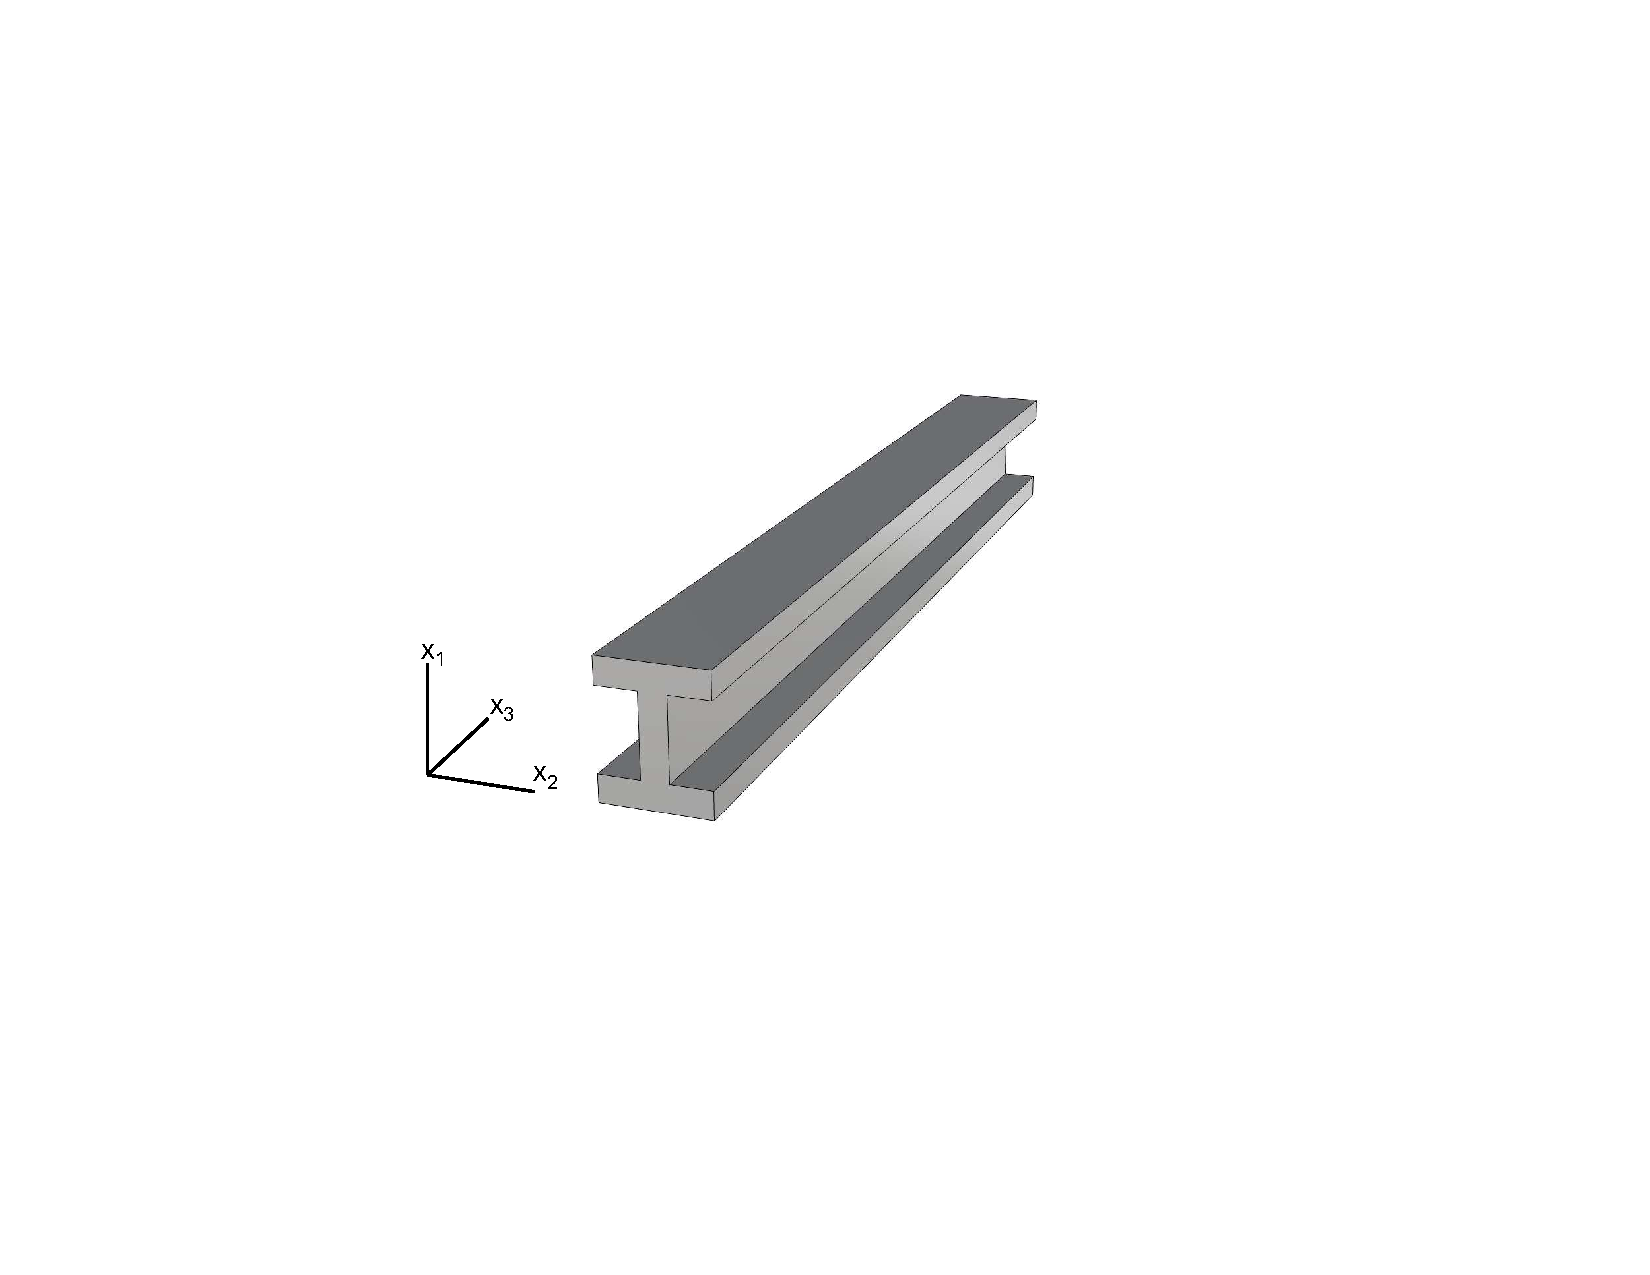
\includegraphics[width=0.2\columnwidth,trim=4cm 7cm 6cm 6.5cm, clip]{figs/straight.pdf}
}
\subfloat[$\theta_3$]{
	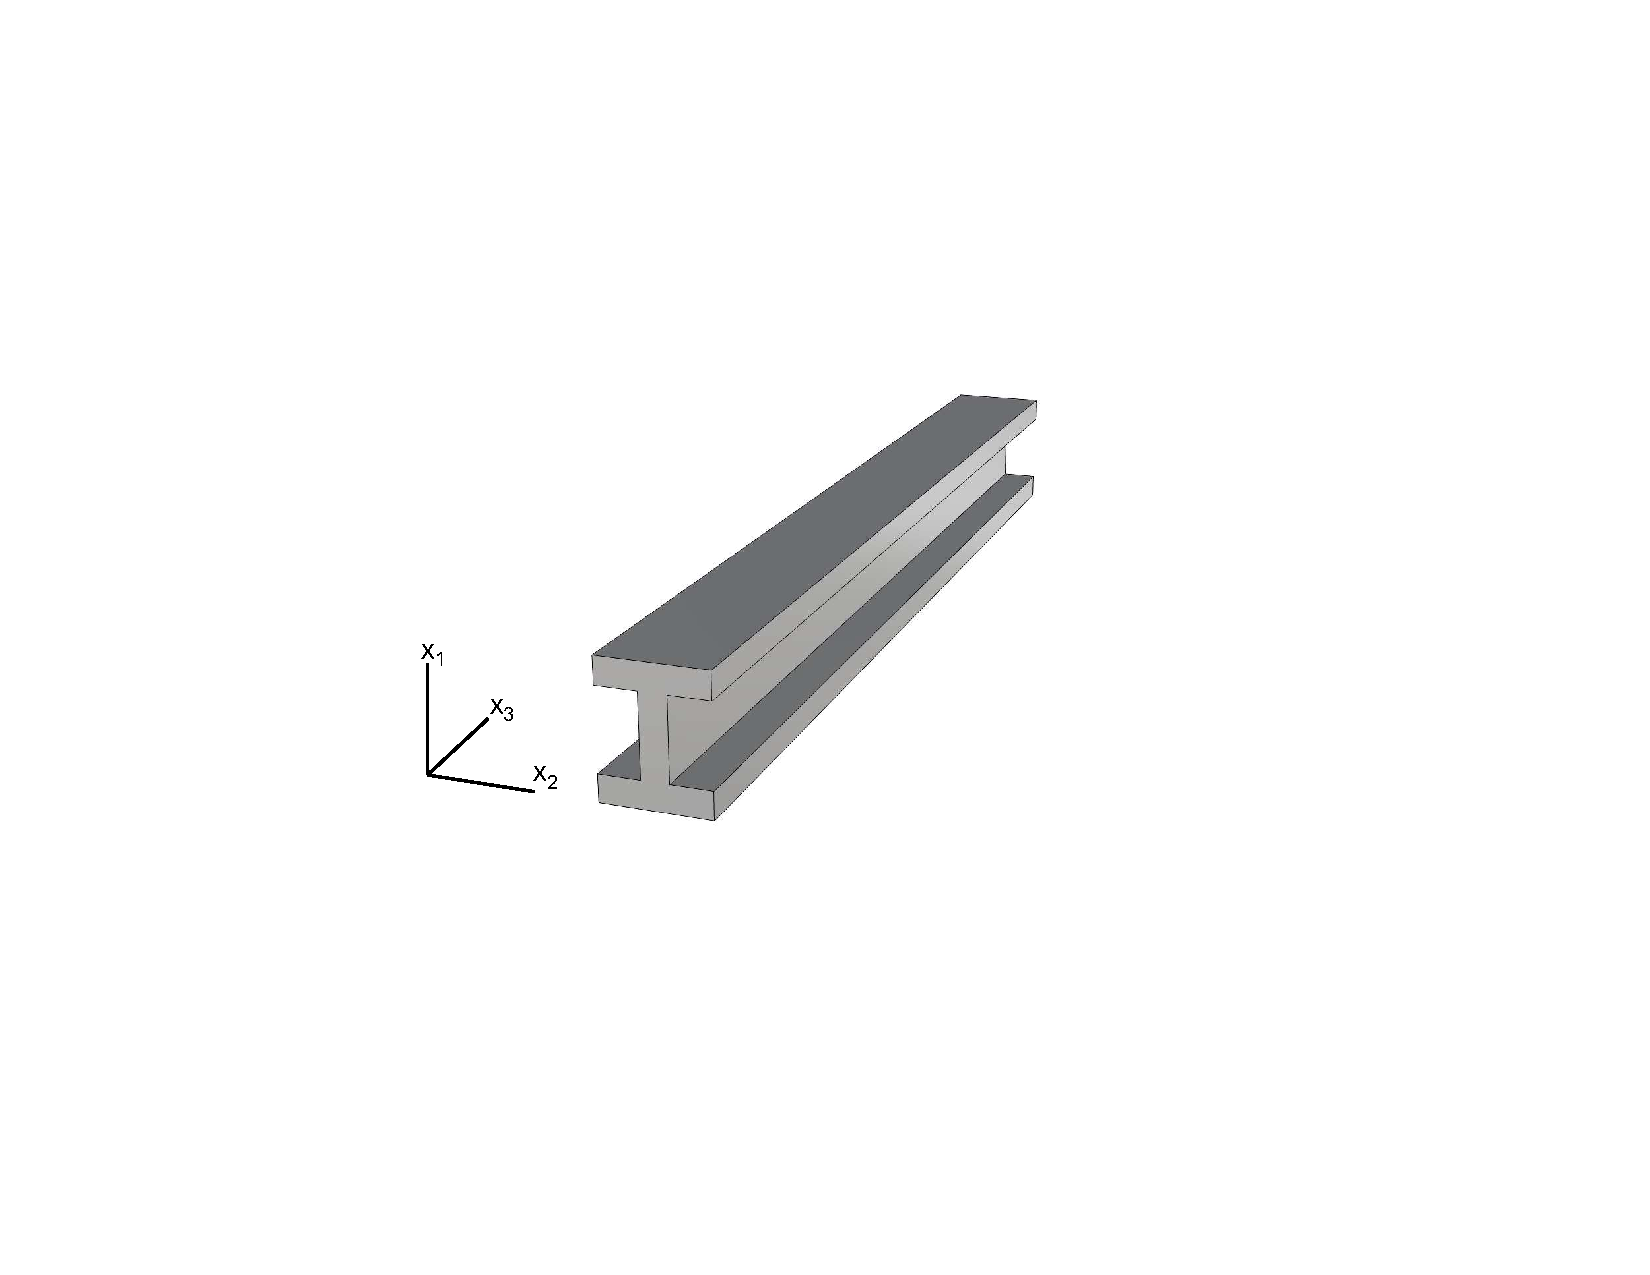
\includegraphics[width=0.2\columnwidth,trim=4cm 7cm 6cm 6.5cm, clip]{figs/straight.pdf}
}
\label{fig:w_theta_displacements}
\caption{Positive displacements in each coordinate direction for both translation and rotation are shown. CHANGE PICTURES}
\end{figure}

Note that in \cref{eq:u1} the $x_2\theta_3(x_3)$ term is subtracted $w_1(x_3)$, while in \cref{eq:u2} $x_1\theta_3(x_3)$ is added to $w_2(x_3)$.
This is an artifact of the positive/negative convection for rotation.
For a point $P$ at some positive valued $(x_1,x_2)$, the $u_1$ displacement is decreased by a $x_3$ rotation.
Similarly for the same point $P$, the $u_2$ displacement is increased by the $\theta_3$ rotation, see \cref{fig:u1u2_plus_minus_xtheta}.
The same sort of scenario occurs in \cref{eq:u3}, see \cref{fig:u3_plus_minus_xtheta}

\begin{figure}
\centering
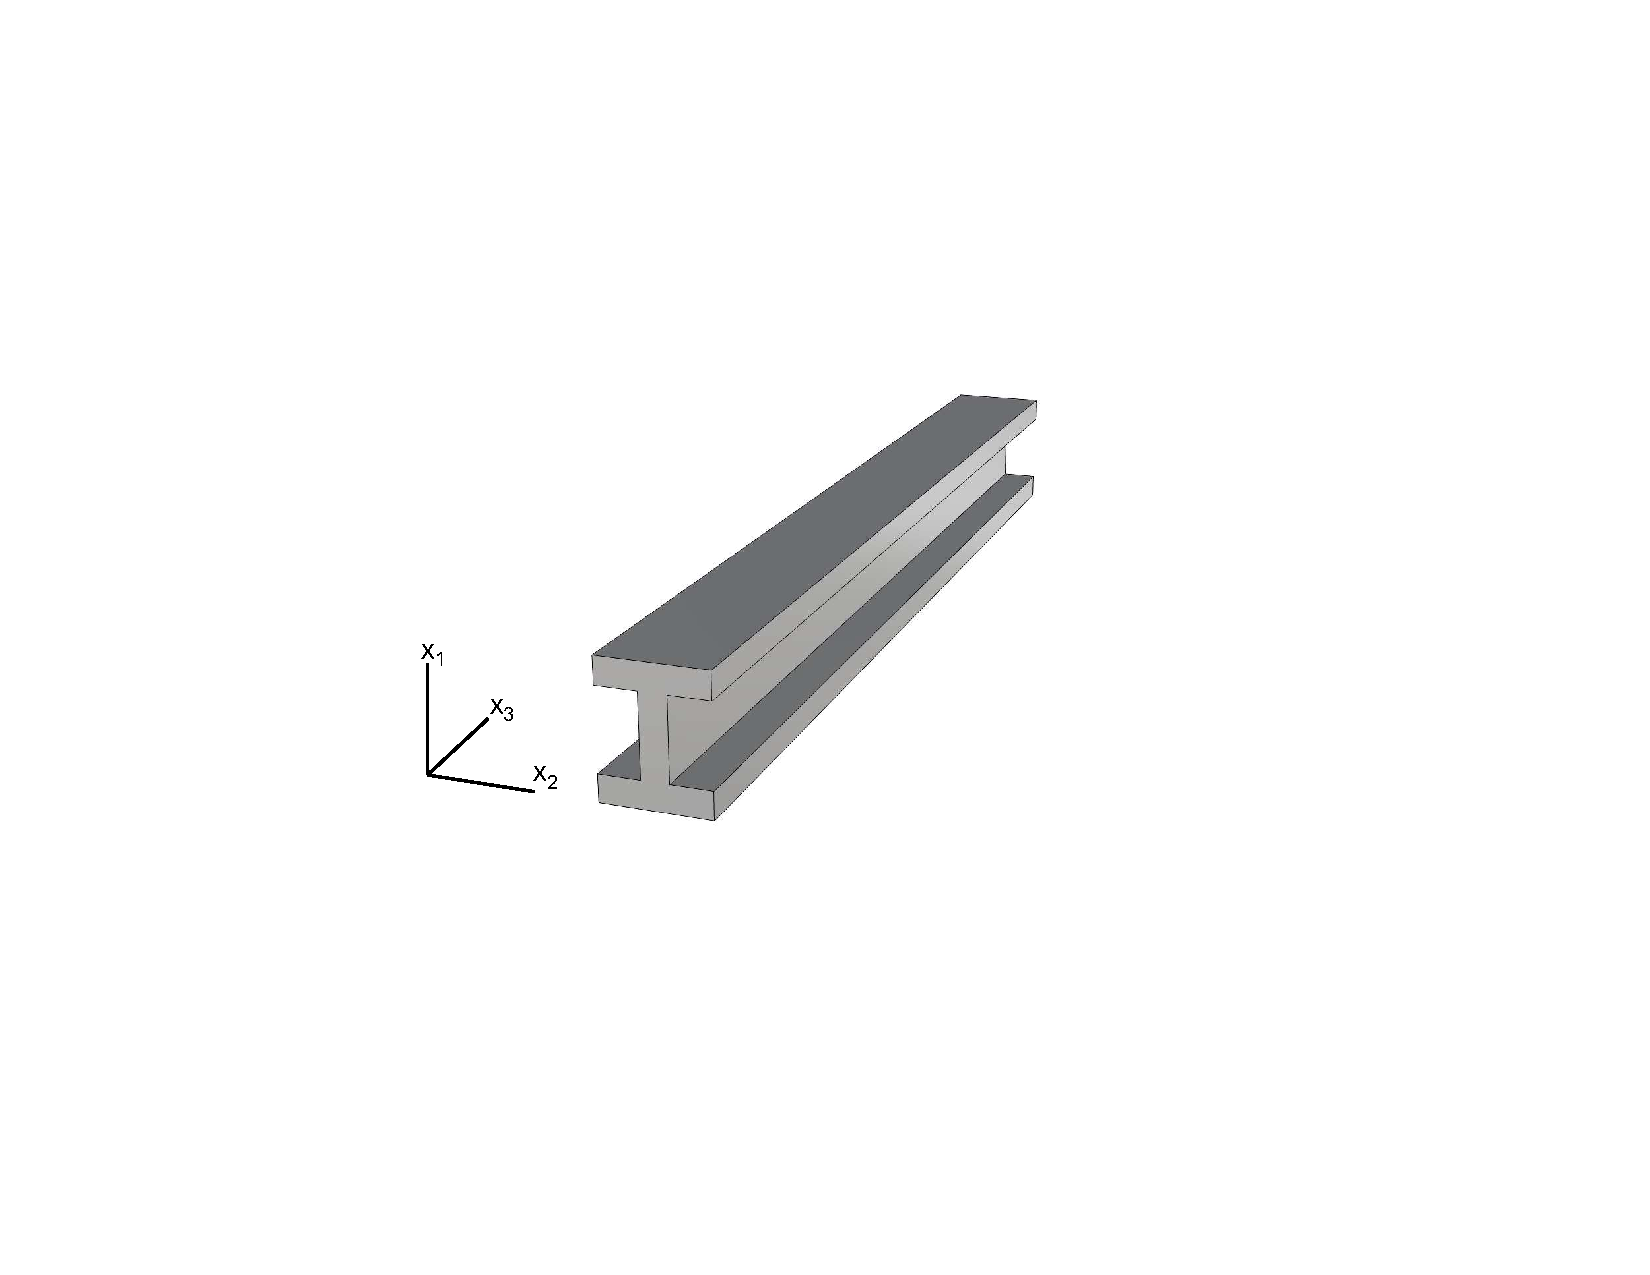
\includegraphics[width=0.2\columnwidth,trim=4cm 7cm 6cm 6.5cm, clip]{figs/straight.pdf}
\caption{A pictoral representation of sign convetion for $\theta_3$ rotations affecting $u_\alpha$ displacements. CHANGE PICTURE}
\label{fig:u1u2_plus_minus_xtheta}
\end{figure}

\begin{figure}
\centering
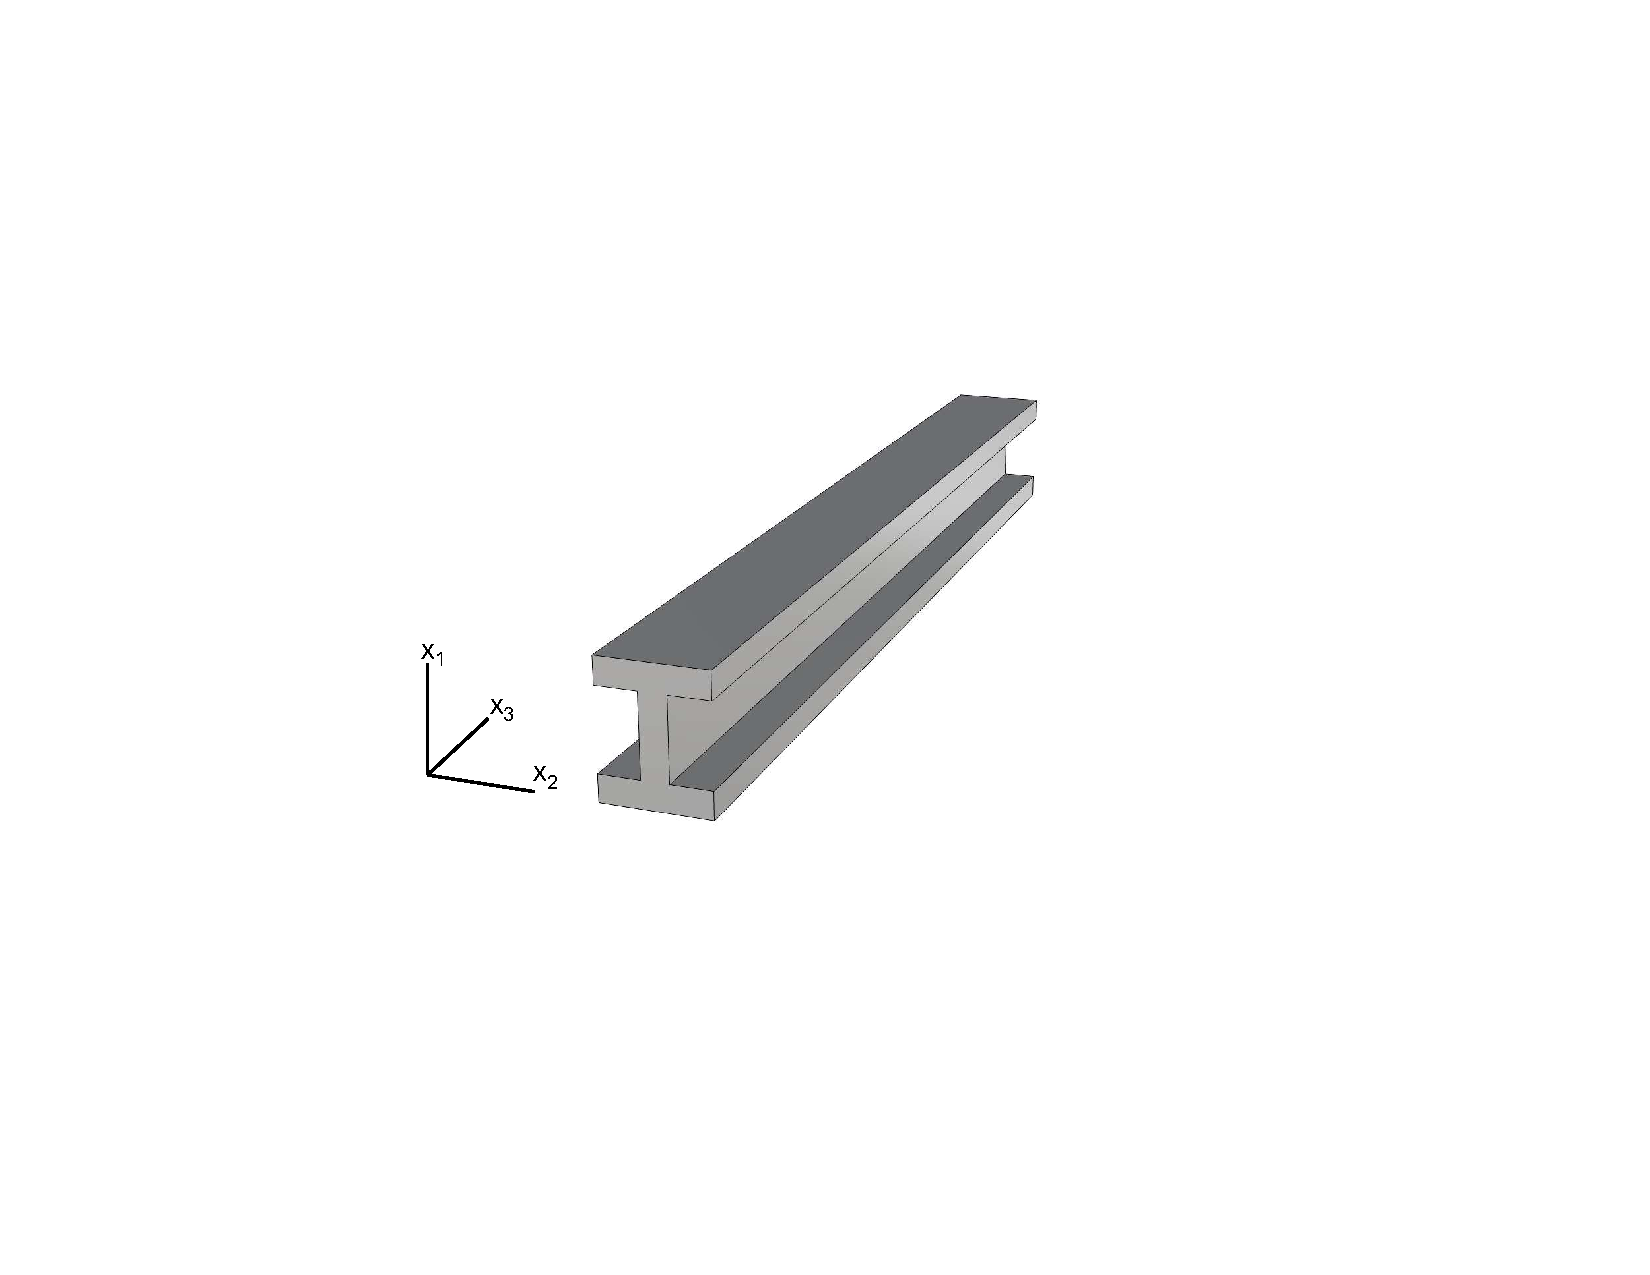
\includegraphics[width=0.2\columnwidth,trim=4cm 7cm 6cm 6.5cm, clip]{figs/straight.pdf}
\caption{A pictoral representation of sign convetion for $\theta_\alpha$ rotations affecting $u_3$ displacements. CHANGE PICTURE}
\label{fig:u3_plus_minus_xtheta}
\end{figure}

It is important to note that the anlysis will be limited or enhanced by the accuracy of these equations.
In this case, warping in the beam is not accounted for.
